\documentclass[12pt, letterpaper]{article}
\usepackage[titletoc,title]{appendix}
\usepackage{color}
\usepackage{booktabs}
\usepackage[usenames,dvipsnames,svgnames,table]{xcolor}
\definecolor{dark-red}{rgb}{0.75,0.10,0.10}
\definecolor{bluish}{rgb}{0.05,0.05,0.85}
\PassOptionsToPackage{unicode}{hyperref}
\PassOptionsToPackage{naturalnames}{hyperref}
\usepackage[margin=1in]{geometry}
\usepackage[linkcolor=blue,
			colorlinks=true,
			urlcolor=blue,
			pdfstartview={XYZ null null 1.00},
			pdfpagemode=UseNone,
			citecolor={bluish},
			pdftitle={partisan}]{hyperref}

%\newcites{SI}{SI References}
\usepackage{natbib}

\usepackage{float}
\usepackage{placeins}

\usepackage{geometry}  % see geometry.pdf on how to lay out the page. There's lots.
\geometry{letterpaper} % This is 8.5x11 paper. Options are a4paper or a5paper or other...
\usepackage{graphicx}  % Handles inclusion of major graphics formats and allows use of
\usepackage{amsfonts,amssymb,amsbsy}
\usepackage{amsxtra}
\usepackage{verbatim}
%\setcitestyle{round,semicolon,aysep={},yysep={;}}
\usepackage{setspace} % Permits line spacing control. Options are:
%\doublespacing
%\onehalfspace
%\usepackage{sectsty}    % Permits control of section header styles
\usepackage{pdflscape}
\usepackage{fancyhdr}   % Permits header customization. See header section below.
\usepackage{url}        % Correctly formats URLs with the \url{} tag
\usepackage{fullpage}   %1-inch margins
\usepackage{multirow}
\usepackage{verbatim}
\usepackage{rotating}
\setlength{\parindent}{3em}

%\usepackage[T1]{fontenc}
%\usepackage[bitstream-charter]{mathdesign}

\usepackage{chngcntr}
\usepackage{longtable}
\usepackage{adjustbox}
\usepackage{dcolumn}

\usepackage[nameinlink, capitalize, noabbrev]{cleveref}

\def\citeapos#1{\citeauthor{#1}'s (\citeyear{#1})}

\makeatother

\usepackage{footmisc}
\setlength{\footnotesep}{\baselineskip}
\makeatother
\renewcommand{\footnotelayout}{\normalsize \doublespacing}


% Colors
\usepackage{color}

\newcommand{\bch}{\color{blue}\em  }   % begin change
\newcommand{\ying} {\color{orange}\em  }   % begin change
\newcommand{\bgcd} {\color{purple}\em }
\newcommand{\ech}{\color{black}\rm  }    % end change

% Caption
\usepackage[hang, font=small,skip=0pt, labelfont={bf}]{caption}
%\captionsetup[subtable]{font=small,skip=0pt}
\usepackage{subcaption}

% tt font issues
% \renewcommand*{\ttdefault}{qcr}
\renewcommand{\ttdefault}{pcr}


\setcounter{page}{0}

\usepackage{lscape}
\renewcommand{\textfraction}{0}
\renewcommand{\topfraction}{0.95}
\renewcommand{\bottomfraction}{0.95}
\renewcommand{\floatpagefraction}{0.40}
\setcounter{totalnumber}{5}
\makeatletter
\providecommand\phantomcaption{\caption@refstepcounter\@captype}
\makeatother


\title{\Large{Holier Than Thou: Partisan Gap in Consumption\\ of Pornography Online}\footnote{You can download the replication materials from \href{http://github.com/soodoku/adult}{https://github.com/soodoku/adult}}}

\author{Lucas Shen\thanks{Lucas is a Research Fellow at Asia Competitiveness Institute, Lee Kuan Yew School of Public Policy, at the National University of Singapore, \href{mailto:lucas@lucasshen.com}{\footnotesize{\texttt{lucas@lucasshen.com}}}} \and Gaurav Sood\thanks{Gaurav can be reached at \href{mailto:gsood07@gmail.com}{\footnotesize{\texttt{gsood07@gmail.com}}}}\vspace{.5cm}}

\date{\today}

\begin{document}
\maketitle

\begin{comment}

setwd("Documents/Github/adult/ms/")
tools::texi2dvi("porn.tex", pdf=TRUE, clean=TRUE) 
setwd(basedir)

\end{comment}

\begin{abstract}
\noindent Consumption of pornography has been blamed for a variety of societal ills, including the rise in misogyny, sex crimes, and the coarsening of culture. Using passively collected browsing data from YouGov, we investigate how much pornography Americans consume online. We find that there is a sharp positive skew in the consumption of pornography, with a small number of users consuming lots of pornography and most consuming small amounts. The median American Internet user today spends X minutes per month consuming pornography, visiting Y sites per month; the 95th percentile is X and Y respectively. Lastly, we find that, unlike previous research \citep{macinnis2015american, edelman2009markets}, which relied on ecological inference, Democrats consume slightly more pornography than Republicans.
\end{abstract} 
\clearpage
\doublespace

Consumption of pornography is associated with a variety of disturbing attitudes, beliefs, emotions, and behaviors. Consuming pornography is associated with support for violence against women \citep{hald2010pornography, malamuth2012pornography, donnerstein1984pornography}, belief in rape myths \citep{foubert2011pornography}, increased gender role conflict, lesser sexual satisfaction \citep{szymanski2014psychological, stewart2012young}, poorer relationship quality \citep{szymanski2014psychological, szymanski2015male}, and sexually risky behaviors such as engaging in paid sex, and having extramarital sex \citep{wright2012internet}. A lot of popular pornography also contains a healthy dose of violence. An analysis of popular pornography revealed that 88.2\% of the scenes contained physical aggression, and 48.7\% verbal aggression \citep{bridges2010aggression}. For all these reasons, there are serious concerns about consumption of pornography.

In this paper, using passive browsing data from YouGov, we investigate how much pornography Americans consume online. We find that there is a sharp skew in the consumption of pornography, with a small set of users consuming a large chunk of pornography. The median American Internet user spends X minutes per month (Y\% of their time online) consuming pornography, visiting Y unique sites; the 95th percentile for time spent consuming pornography online is YY minutes.

We also use the data to shed light on an age-old debate --- whether Democrats consume more pornography than Republicans or vice versa. Both parties claim the higher moral ground. And in surveys both parties think consumption of pornography is abhorrent, plausibly for different reasons. Unlike previous research, which relied on ecological inference, we find that Democrats consume slightly more pornography online than Republicans \citep{macinnis2015american, edelman2009markets}. Adjusting for background covariates like age, gender etc., further mutes the differences.

\section*{Data}
We use passively observed browsing data from a YouGov survey to measure the consumption of adult content. YouGov maintains a large online panel recruited through a variety of methods. It uses matched sampling to survey respondents: The provider first draws a random sample from a large synthetic representative sampling frame, finds respondents that match the sampled individuals from its panel, and invites them to take a survey. For details and validation, see \citet{rivers2009}. For this particular sample, panelists also provided de-identified access to their web browsing activity via passive metering software installed voluntarily on their computers. The software, called RealityMine, can be uninstalled at any point and captures visited web URLs independent of the type of browser or browser-specific privacy settings.\footnote{RealityMine does not save passwords or financial transactions, and personally identifying information is screened out by the survey provider.} At the time this data was made available in June, 2022, YouGov had recruited 1,200 individuals to the web tracking panel, which is currently marketed as YouGov Pulse. The passive metering component of this particular opt-in panel adds a layer of selectivity to the sampling process. 

Overall, we have over 6 million web browsing records by the 1,200 individuals over the one-month period of June 2022. 
For each web browsing activity, we have information on the domain (e.g., wikipedia.org), the time of visit, and the time spent on the domain. Individuals are spread out over the US states and regions (see \cref{fig:map_duration}). 
Our data also comes with characteristics for the 1,200 individuals.
We have information on their party identification, which we use to code their partisanship.
We verify this using information on whether they voted for the Republican or Democratic candidate in the 2020 presidential election.
Most individuals reported their party identification, with 120 individuals who did not respond or say not sure/don't know.
Out of the 1,080 individuals who report party identification, the majority 82 percent lean either Republican or Democrat. The remaining 18 percent identify as independent.
In the analyses focusing on splits by party, we use only those who lean either Republican or Democrat.
We also have information on birth year, gender, race, and education level.
\cref{tab:characteristics_split_by_party} shows differences in gender, and race(?) by party. 
Hence, our analyses below for differences in porn consumption includes these characteristics in the estimation.




\section*{Measuring Consumption of Adult Content}
For YouGov, we only observe data from a single machine per person. Our analyses should hold if people exhibit similar consumption patterns across devices. If that is too implausible an assumption, then we must decide on the direction of error and how it affects our analyses. We think it is likely that people would be less likely to search for pornography on machines on which they have installed passive monitoring software (though the data are de-identified). If that is so, our estimates are a lower bound of net consumption of pornography per machine. As the number of devices per person is increasing, all these numbers need to be adjusted. Next, is measurement error correlated with ideology? We have little reason to expect that, but we have no capacity to check if it is true. Thus, for current purposes, we assume that it is so.  

We code pornographic content at the domain level. 
Our main analysis depends on the domain classifications that come with YouGov data. We code domains that YouGov categorizes as ``Adult'' as porn sites. 
These include ``Adult'' (e.g., xvideos.com), ``Adult, Business'' (e.g., onlyfans.com), and ``Adult, Entertainment'' (e.g., hentainfox.com). 
A fraction of web browsing activity, approximately 84k or 1.3 percent, are to porn sites.
See \cref{fig:top25_adult} and \cref{fig:top25_nonadult} for the top visited domains.
Certain domains are not predominately for porn consumption and we remove these from the classification of porn sites. For instance, urbandictionary.com and 4chan.org are ``Adult'' but not classified as porn site.\footnote{We manually check the top adult domains in our sample to remove obvious false positives. Generally, if there is graphic nudity on the landing page or if the site is some form of erotica, we classify the site as a porn site.}
In the Appendix, we use a keyword classifier and a machine learning classifier. As you will see, all of these methods consistently show the same thing. All of this ignores pornography available via more conventional channels. For instance, some pornography is consumed on sites like Tumblr.

The consumption of pornography is concentrated. Traffic to the top 10 most frequented porn sites more than 12 times that of traffic to all other porn sites outside the top 10 (approximately 109 minutes vs 9 minutes, see \crefrange{fig:concentration_porn_consumption}{fig:concentration_porn_consumption_by_party}). 
For panelists who consume porn, close to 80 percent of their traffic to adult sites is concentrated in just one porn site (\cref{fig:concentration_porn_consumption_topX_by_party}). This behavior does not differ substantially party.

\FloatBarrier
\section*{Results}

Our primary dependent variables of interest are: total time spent on pornographic sites and the proportion of time spent on pornographic sites. (In the appendix, we show similar analysis for visits.) 


%======================================================
% Figure for Distribution of Hours spent on adult sites
%======================================================
\begin{figure}[ht]
\centering
\caption{Distribution of Consumption of Pornography Online}
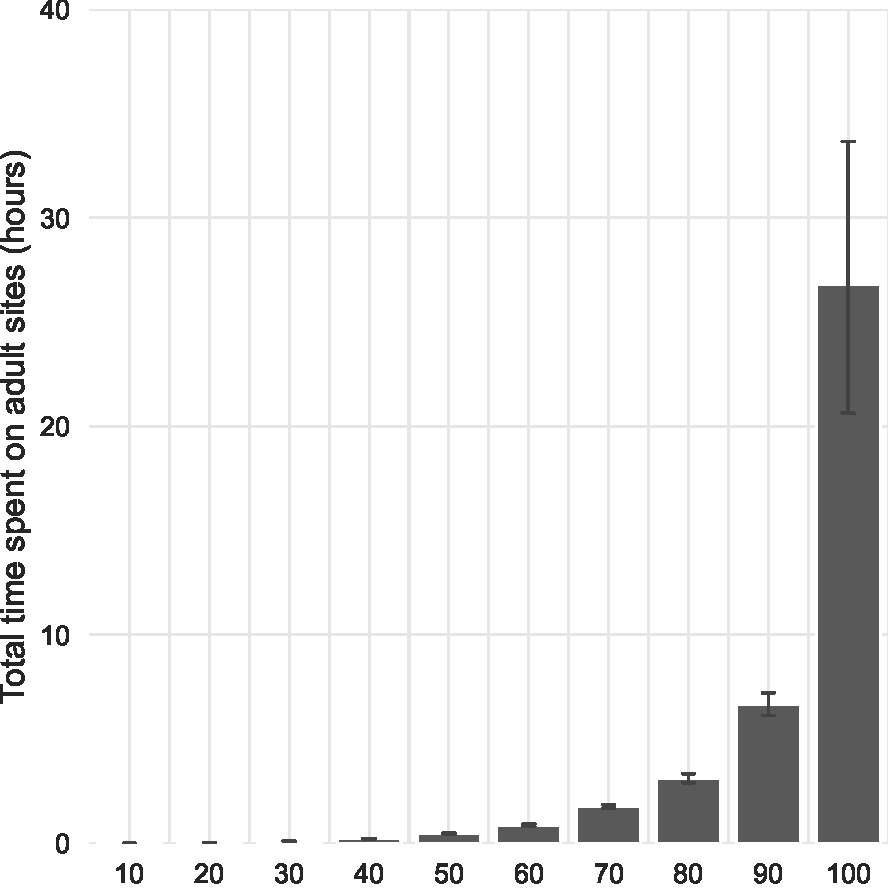
\includegraphics[width=.5\linewidth]{../figs/distribution_duration_on_adultsites.pdf}
\caption*{\footnotesize \emph{Notes:} 
	Figure shows the number of hours spent on adult sites by individuals who consumed pornography in the sample period.
	Individuals are split into deciles with each bin containing approximately the same number of individuals.
	Height of bars indicate mean of each bin.
	Capped vertical bars are 95\% confidence intervals.
	See \cref{tab:distribution_duration} for the more tabulated values.
}
\label{fig:distribution_duration}
\end{figure}

%===================================================================
% Figure for Distribution of proportion of time spent on adult sites
%===================================================================
\begin{figure}[ht]
	\centering
	\caption{Percentage of Time Spent on Pornographic Sites}
	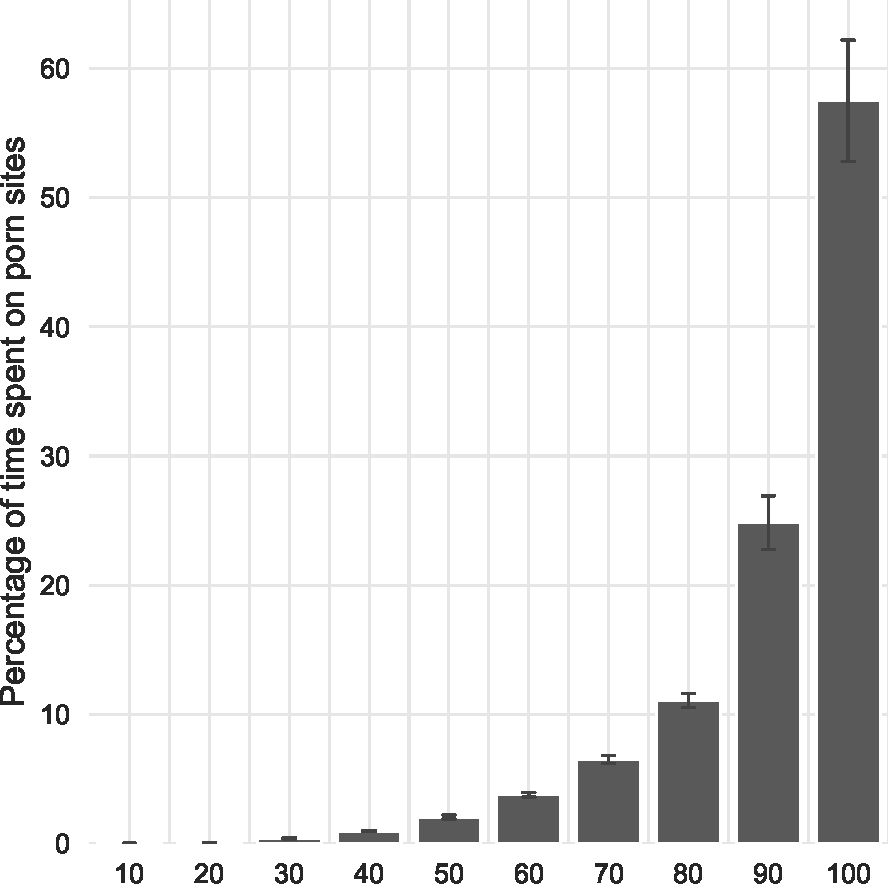
\includegraphics[width=.5\linewidth]{../figs/distribution_proportion_duration_on_adultsites.pdf}
	\caption*{\footnotesize \emph{Notes:} 
		Figure shows the proportion of time spent on adult sites by individuals who consumed pornography in the sample period.
		Individuals are split into deciles with each bin containing approximately the same number of individuals.
		Height of bars indicate mean of each bin.
		Capped vertical bars are 95\% confidence intervals.
		See \cref{tab:distribution_prop_duration} for the more tabulated values.
	}
	\label{fig:distribution_prop_duration}
\end{figure}



%===============================================
% Splits by party for hours spent on adult sites
%===============================================
\begin{figure}[ht]
	\centering
	\caption{Distribution of Consumption of Pornography Online by Party}
	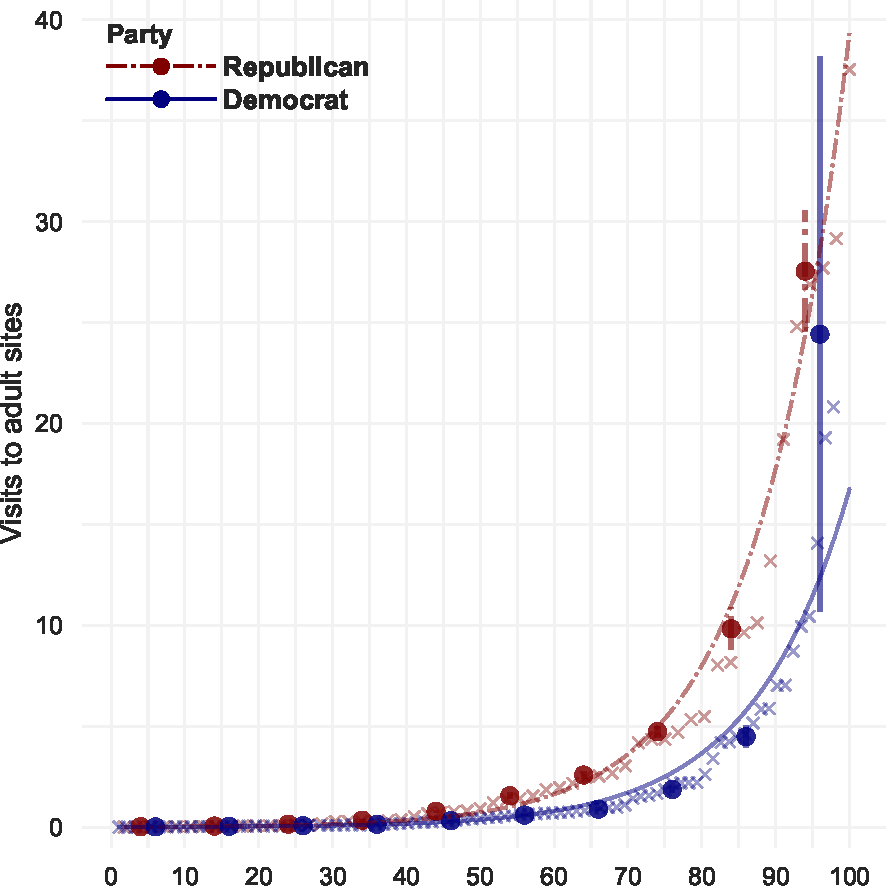
\includegraphics[width=.6\linewidth]{../figs/distribution_duration_on_adultsites_by_party.pdf}
	\caption*{\footnotesize \emph{Notes:} 
		Figure shows splits by party and by percentiles for the total time spent on adult sites for panelists in the sample who consumed pornography in the sample period.
		Round markers and the corresponding vertical lines indicate the mean and 95\% confidence intervals for each bin.
		The \emph{x} symbols indicate actual panelists based on their percentiles.
		See \cref{tab:distribution_duration_party} for the more tabulated values.
	}
	\label{fig:distribution_duration_party}
\end{figure}


%============================================================
% Splits by party for proportion of time spent on adult sites
%============================================================
\begin{figure}[ht]
	\centering
	\caption{Percentage of Time Spent on Pornographic Sites by Party}
	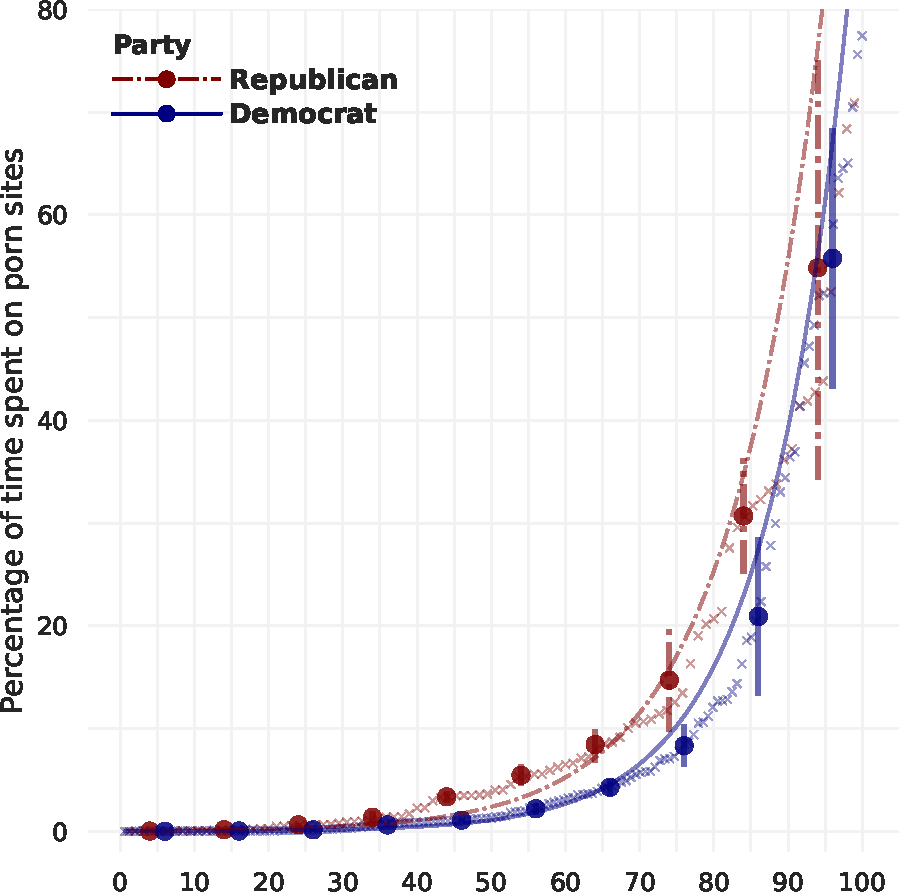
\includegraphics[width=.6\linewidth]{../figs/distribution_proportion_duration_on_adultsites_by_party.pdf}
	\caption*{\footnotesize \emph{Notes:} 
		Figure shows splits by party and by percentiles for the proportion of time spent on adult sites for panelists in the sample who consumed pornography in the sample period.
		Round markers and the corresponding vertical lines indicate the mean and 95\% confidence intervals for each bin.
		The \emph{x} symbols indicate actual panelists based on their percentiles.
		See \cref{tab:distribution_prop_duration_party} for the more tabulated values.
	}
	\label{fig:distribution_prop_duration_party}
\end{figure}


\newpage


To formally test for these differences, we ran quantile regression, regressing the duration on party. 

%===========================
% Quantile regressions
% Hours spent on adult sites
%===========================
\begin{figure}[ht]
\centering
\caption{Quantile Estimates--Hours Spent on Adult Sites by Party}
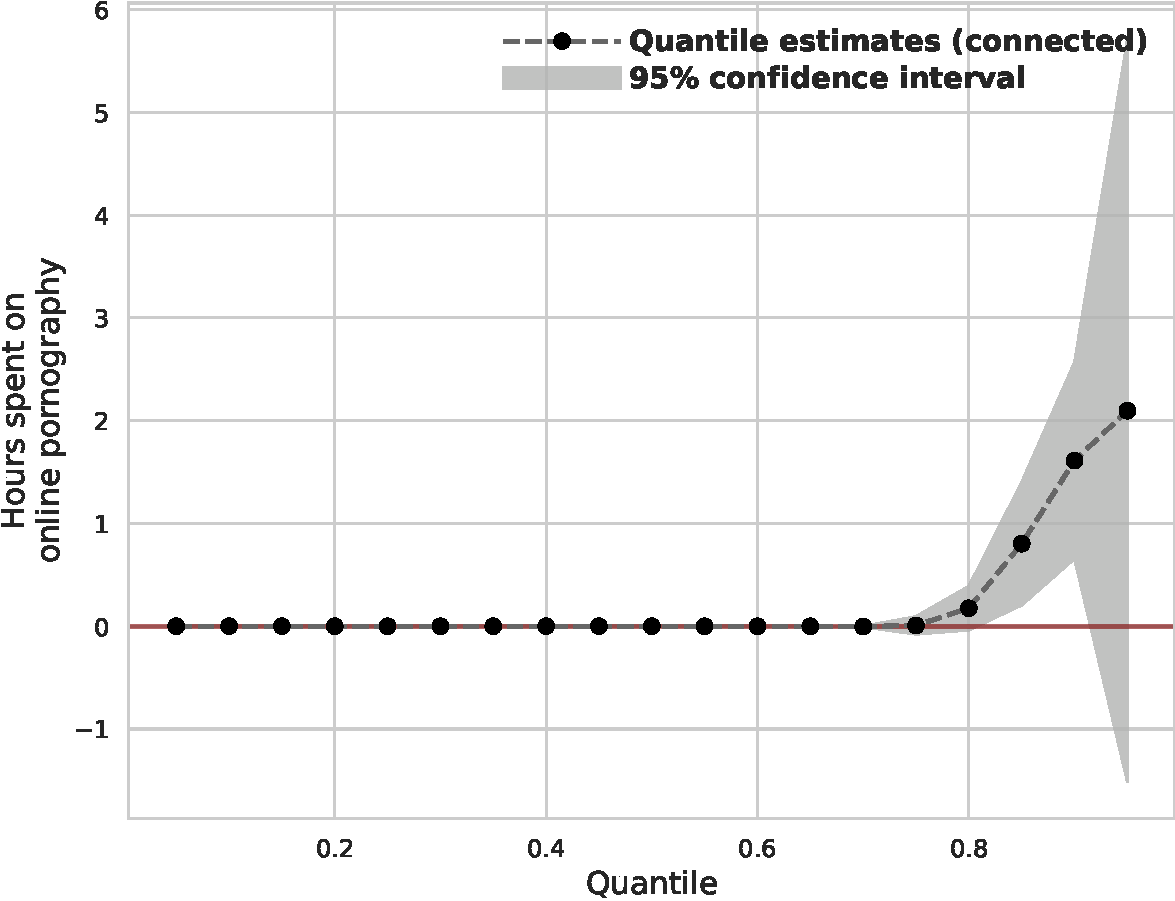
\includegraphics[width=.6\linewidth]{../figs/quantile_reg_duration_adult.pdf}
	\caption*{\footnotesize \emph{Notes:} 
		Dependent variable is the number of hours panelists in our sample spent on adult sites.
		Each point indicates the difference between Republicans and Democrats and corresponds to a quantile regression at the quantile indicated by the x-axis.
		95\% confidence intervals constructed from robust standard errors.
		See \cref{fig:quantile_regression_duration_covariates} for the same plot controlling for individual characteristics.
}
\label{fig:quantile_regression_duration}
\end{figure}

%========================================
% Quantile regressions
% Proportion of time spent on adult sites
%========================================
\begin{figure}[ht]
	\centering
	\caption{Quantile Estimates--Percentage of Time Spent on Adult Sites by Party}
	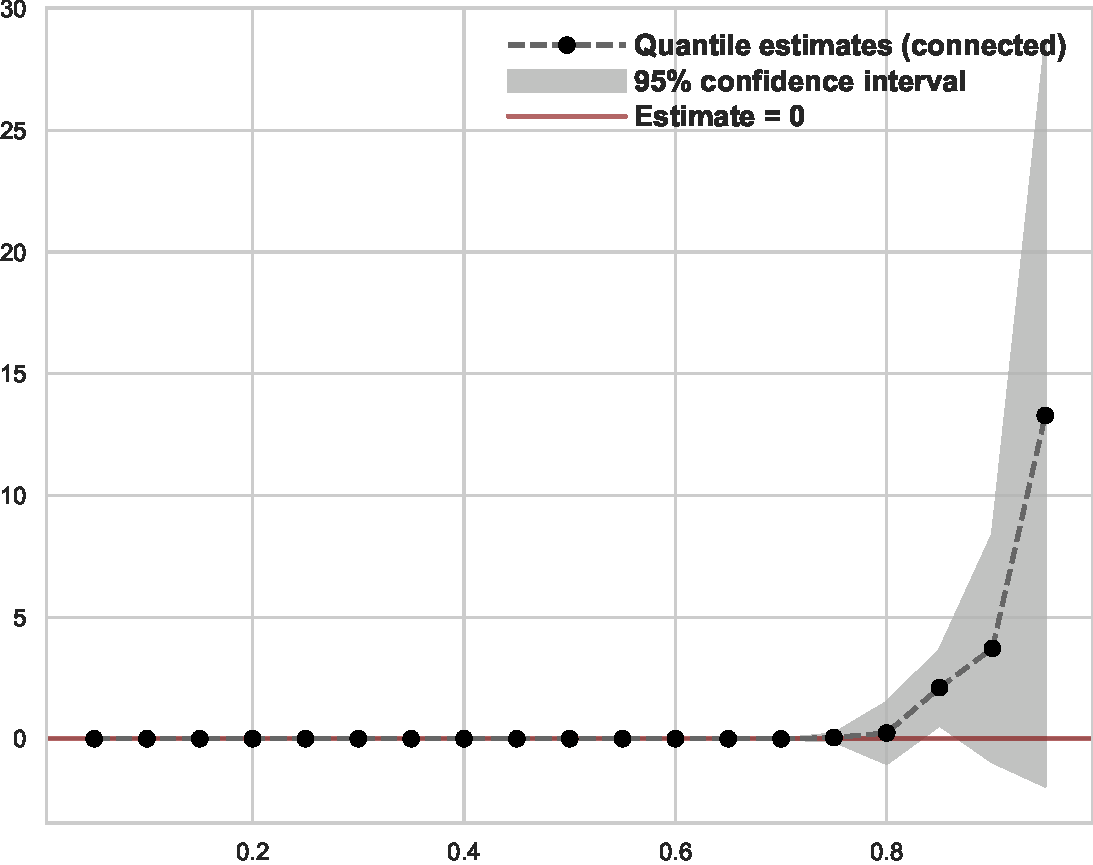
\includegraphics[width=.6\linewidth]{../figs/quantile_reg_proportion_duration_adult.pdf}
	\caption*{\footnotesize \emph{Notes:} 
		Dependent variable is the percentage of time panelists in our sample spent on adult sites.
		Each point indicates the difference between Republicans and Democrats and corresponds to a quantile regression at the quantile indicated by the x-axis.
		95\% confidence intervals constructed from robust standard errors.
		See \cref{fig:quantile_regression_prop_duration_covariates} for the same plot controlling for individual characteristics.
	}
	\label{fig:quantile_regression_prop_duration}
\end{figure}


\newpage

These minor differences (or lack of differences) could be because of the demographic differences we see across the party. This lack of difference also partly stems from a lack of difference in the tendency to consume pornography (see \cref{fig:consume_porn_yes_no}). Next, we control for immutable characteristics like age and gender to see if that adjustment changes the picture much. Given how concentrated pornographic consumption is in our data, it is unlikely to make much of a difference and that is indeed what we find. 



\section*{Discussion}
Consumption of pornography is also problematic from a religious perspective. Christian theologians believe that consumption of pornography leads people away from purity and hence should be avoided.\footnote{\url{https://www.churchofjesuschrist.org/study/manual/help-for-pornography-users/effect-of-pornography}}.
\clearpage
\bibliographystyle{apsr}
\bibliography{porn}
\clearpage

%===============================================================================
%===============================================================================
% Appendix
%===============================================================================
%===============================================================================
\appendix
\renewcommand{\thesection}{SI \arabic{section}}
\renewcommand\thetable{\thesection.\arabic{table}}  
\renewcommand\thefigure{\thesection.\arabic{figure}}
\counterwithin{figure}{section}
\counterwithin{table}{section}
\begin{center}
\Large{Supporting Information}
\end{center}

\FloatBarrier
%===============================================================================
% Supplementary Descriptives for sense of landscape of porn consumption
%===============================================================================
\section{Supplementary Descriptive Figures and Tables}
%============================
% Figure of top 25 adultsites
%============================
\begin{figure}[ht]
	\centering
	\caption{Top 25 Adult Domains}
	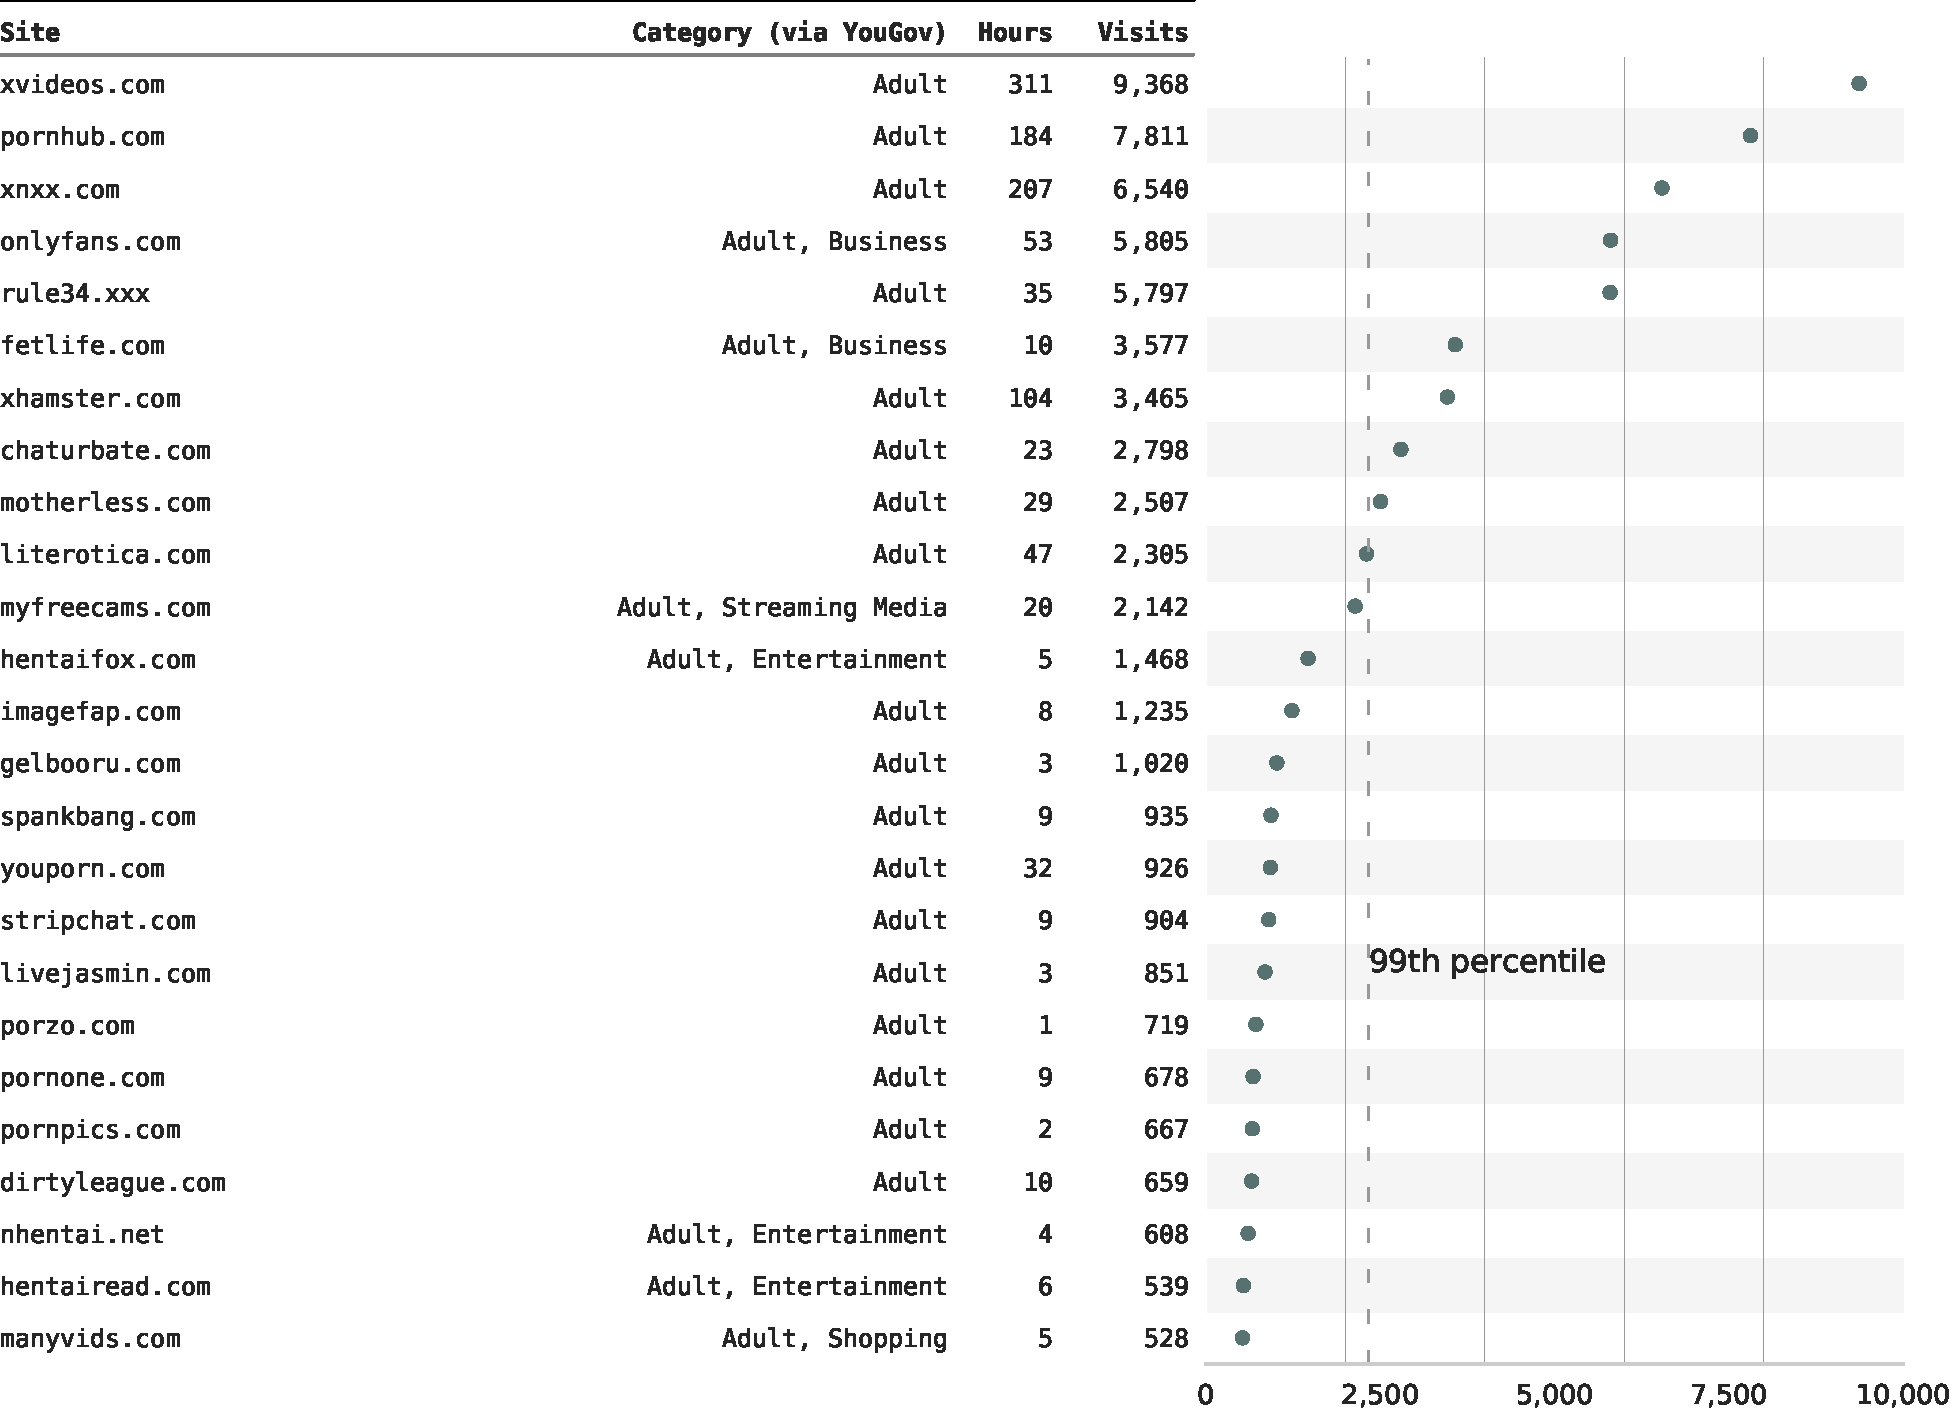
\includegraphics[width=\textwidth]{../figs/top_25_adultsites.pdf}
	\caption*{\footnotesize \emph{Notes:} 
		Table shows the top 25 adult sites that panelists visit in the sample period.
		Adult sites are categorized by YouGov.
		The \emph{Hours} column are the total number of hours that panelists in the sample spent on the site. 
		The \emph{Visits} column is total number of visits by panelists in the sample to the site.  
		Sites to the right of the vertical dashed are the top 1 percent.
	}
	\label{fig:top25_adult}
\end{figure}

%================================
% Figure of top 25 non-adultsites
%================================
\begin{figure}
	\centering
	\caption{Top 25 (Non-Adult) Domains}
	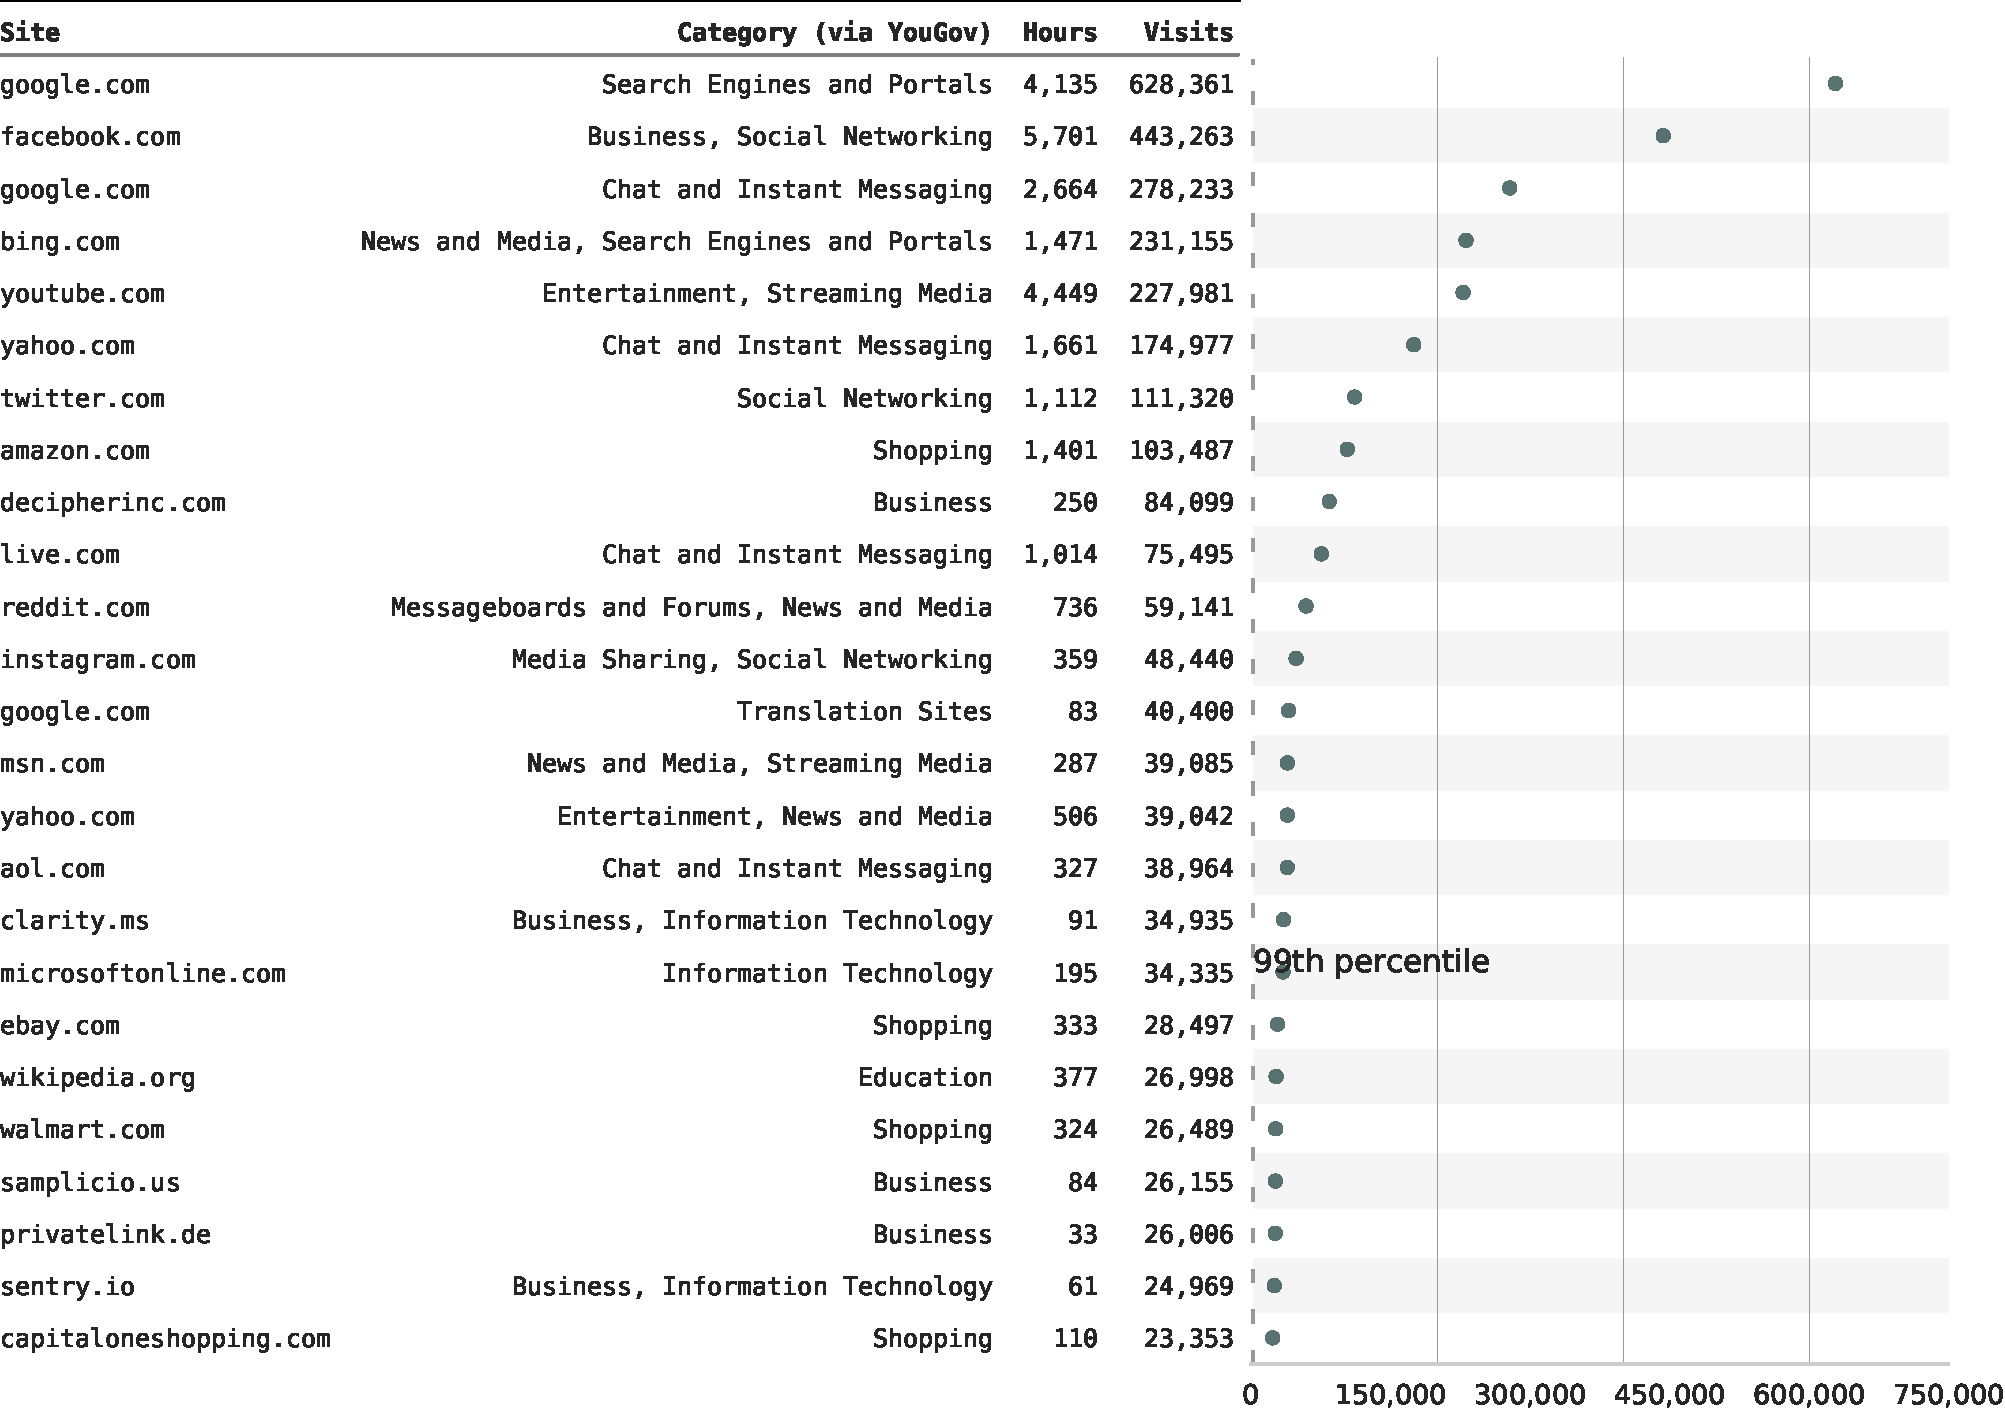
\includegraphics[width=\textwidth]{../figs/top_25_nonadultsites.pdf}
	\caption*{\footnotesize \emph{Notes:} 
		Table shows the top 25 non-adult sites that panelists visit in the sample period.
		The \emph{Hours} column are the total number of hours that panelists in the sample spent on the site. 
		The \emph{Visits} column is total number of visits by panelists in the sample to the site.  			
		Sites to the right of the vertical dashed are the top 1 percent.
	}
	\label{fig:top25_nonadult}
\end{figure}


%=============================================
% Figure for concentration of porn consumption
%=============================================
\begin{figure}
	\centering
	\caption{Traffic to Top 10 Porn Sites}
	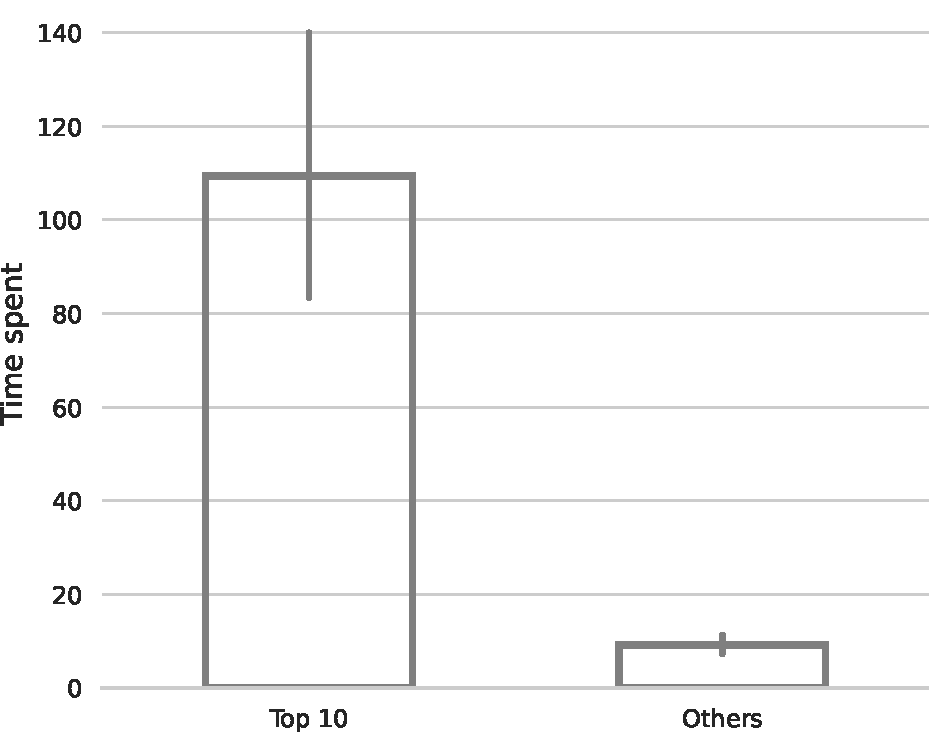
\includegraphics[width=.5\textwidth]{../figs/concentration_porn_consumption.pdf}
	\caption*{\footnotesize \emph{Notes:} 
		The Top 10 bar indicates traffic to the top 10 adult sites in the data (see \cref{fig:top25_adult}).
		Time units is hours.
		Data is at the panelist-domain level.
		Others indicate traffic to all other adult sites outside of the top 10.
		Vertical bars are 95\% confidence intervals from bootstrapped standard errors (n = 1,000).
	}
	\label{fig:concentration_porn_consumption}
\end{figure}

%======================================================
% Figure for concentration of porn consumption by party
%======================================================
\begin{figure}
	\centering
	\caption{Traffic to Top 10 Porn Sites by Party}
	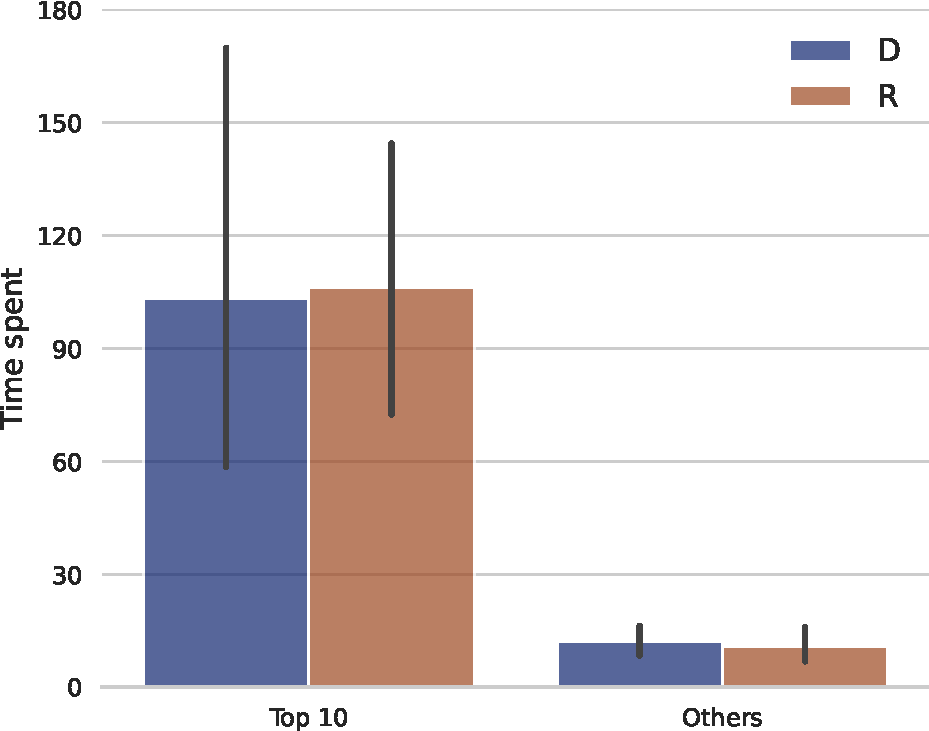
\includegraphics[width=.6\textwidth]{../figs/concentration_porn_consumption_by_party.pdf}
	\caption*{\footnotesize \emph{Notes:} 
		The Top 10 bar indicates traffic to the top 10 adult sites in the data (see \cref{fig:top25_adult}).
		Time units is hours.
		Data is at the panelist-domain level.
		Others indicate traffic to all other adult sites outside of the top 10.
		Vertical bars are 95\% confidence intervals from bootstrapped standard errors (n = 1,000).
	}
	\label{fig:concentration_porn_consumption_by_party}
\end{figure}

%====================================
% Figure of traffic to top x websites
%====================================
\begin{figure}
	\centering
	\caption{Traffic to Top x Porn Sites by Party}
	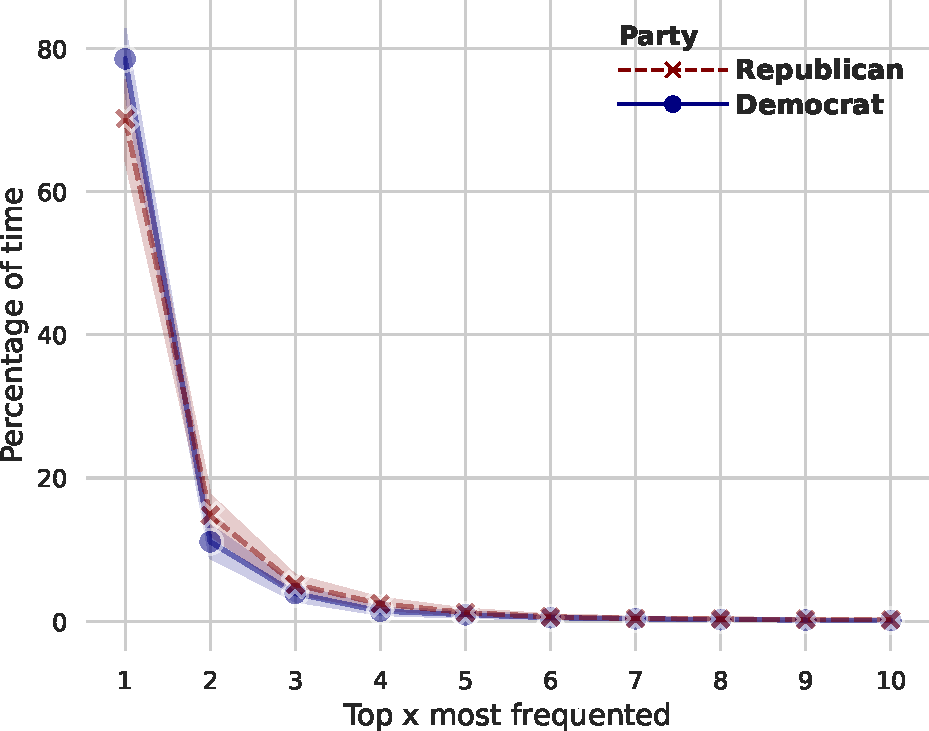
\includegraphics[width=.6\textwidth]{../figs/concentration_porn_consumption_topX_by_party.pdf}
	\caption*{\footnotesize \emph{Notes:} 
		Figure shows concentration of porn consumption based on individuals' most frequented porn sites.
		Shaded areas are 95\% confidence intervals from bootstrapped standard errors (n = 1,000).
	}
	\label{fig:concentration_porn_consumption_topX_by_party}
\end{figure}


%============================================================================
% Figure of porn consumption by party
% Y-axis = proportion of individuals that ever consumed porn in sample period
%============================================================================
\begin{figure}
	\centering
	\caption{Porn Consumption by Party}
	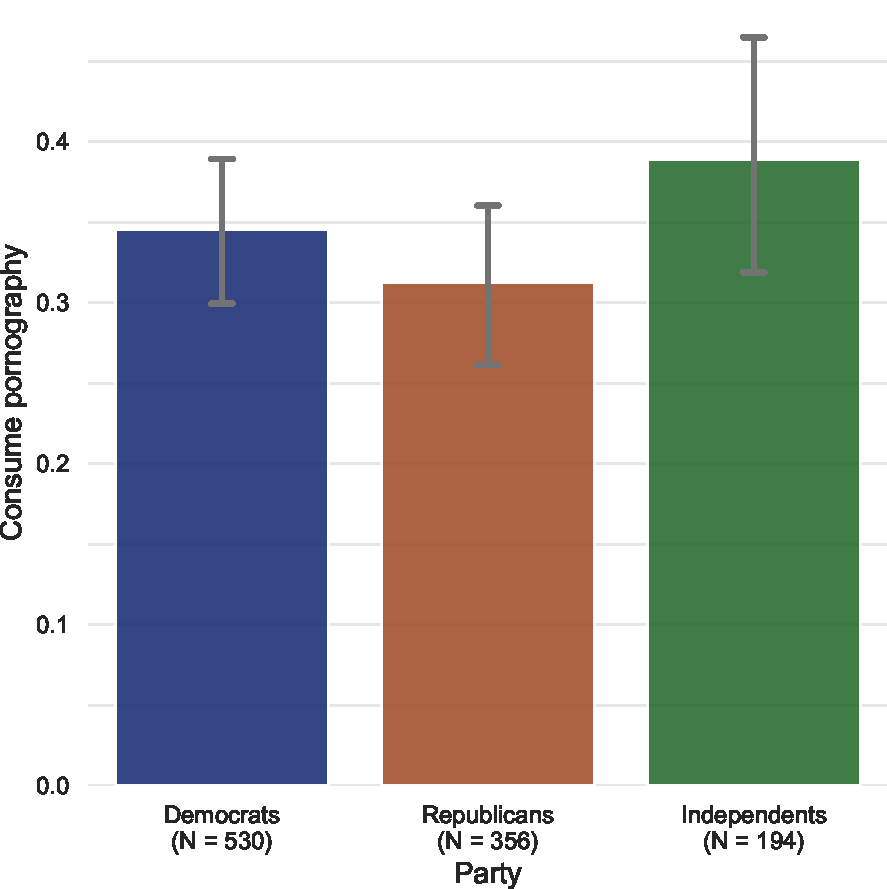
\includegraphics[width=.5\textwidth]{../figs/consume_porn_yes_no.pdf}
	\caption*{\footnotesize \emph{Notes:} 
		Figure shows proportion of panelists in the sample who ever consumed pornography in the sample period by party.
		Capped vertical bars are 95\% confidence intervals from bootstrapped standard errors (n = 1,000).
	}
	\label{fig:consume_porn_yes_no}
\end{figure}


%====================================================
% Tabulated percentiles of hours spent on adult sites
%====================================================
\begin{table}[ht] \centering \small \setlength\tabcolsep{10 pt}
	\caption{Distribution of Consumption of Pornography Online}
	\label{tab:distribution_duration}
	\begin{adjustbox}{max width=\textwidth}
		\begin{tabular}{cr}
			\toprule
			\multicolumn{1}{c}{\textbf{Percentile}}&\multicolumn{1}{c}{\textbf{Hours}}\\
			\midrule
			0.00 &  0.00 \\
0.10 &  0.02 \\
0.20 &  0.07 \\
0.30 &  0.16 \\
0.40 &  0.33 \\
0.50 &  0.64 \\
0.60 &  1.30 \\
0.70 &  2.20 \\
0.80 &  4.49 \\
0.90 & 10.15 \\
0.95 & 19.50 \\
0.96 & 21.93 \\
0.97 & 27.31 \\
0.98 & 32.22 \\
0.99 & 46.47 \\
1.00 & 93.96 \\\\
			\bottomrule
		\end{tabular}
	\end{adjustbox}
	\caption*{\footnotesize \emph{Notes:} 
		Table shows key percentiles (each of the ten deciles plus quantiles at the right tail) and their corresponding values for the duration (hours) spent by individuals who consumed pornography in the sample period. 
		See \cref{fig:distribution_duration} for the plot.
	}
\end{table}

%=====================================================================
% Tabulated percentiles of proportion of duration spent on adult sites
%=====================================================================
\begin{table}[ht] \centering \small \setlength\tabcolsep{10 pt}
	\caption{Percentage of Time Spent on Pornographic Sites}
	\label{tab:distribution_prop_duration}
	\begin{adjustbox}{max width=\textwidth}
		\begin{tabular}{cr}
			\toprule
			\multicolumn{1}{c}{\textbf{Percentile}}&\multicolumn{1}{c}{\textbf{Hours}}\\
			\midrule
			0.00 &  0.0 \\
0.10 &  0.0 \\
0.20 &  0.1 \\
0.30 &  0.5 \\
0.40 &  1.0 \\
0.50 &  2.4 \\
0.60 &  4.3 \\
0.70 &  7.9 \\
0.80 & 13.5 \\
0.90 & 34.3 \\
0.95 & 55.6 \\
0.96 & 62.8 \\
0.97 & 64.3 \\
0.98 & 68.9 \\
0.99 & 73.9 \\
1.00 & 87.5 \\
			\bottomrule
		\end{tabular}
	\end{adjustbox}
	\caption*{\footnotesize \emph{Notes:} 
		Table shows key percentiles (each of the ten deciles plus quantiles at the right tail) and their corresponding values for the duration (hours) spent by individuals who consumed pornography in the sample period. 
		See \cref{fig:distribution_prop_duration} for the plot.
	}
\end{table}

%===========================================================================
% Tabulated splits by party and by percentiles for hours spent on adultsites
%===========================================================================
\begin{table}[ht] \centering \small \setlength\tabcolsep{10 pt}
	\caption{Distribution of Consumption of Pornography Online by Party}
	\label{tab:distribution_duration_party}
	\begin{adjustbox}{max width=\textwidth}
		\begin{tabular}{crr}
			\toprule
			\multicolumn{1}{l}{\textbf{Percentile}}&\multicolumn{1}{c}{\textbf{Republicans}}&\multicolumn{1}{r}{\textbf{Democrats}}\\
			\midrule
			0.00 &  0.00 &  0.00 \\
0.10 &  0.04 &  0.02 \\
0.20 &  0.12 &  0.05 \\
0.30 &  0.29 &  0.11 \\
0.40 &  0.58 &  0.18 \\
0.50 &  1.36 &  0.38 \\
0.60 &  2.11 &  0.69 \\
0.70 &  3.04 &  1.37 \\
0.80 &  5.51 &  3.41 \\
0.90 & 11.57 &  7.15 \\
0.95 & 24.91 & 15.57 \\
0.96 & 26.91 & 17.33 \\
0.97 & 27.74 & 19.28 \\
0.98 & 29.30 & 21.65 \\
0.99 & 36.59 & 43.01 \\
1.00 & 37.54 & 90.48 \\\\
			\bottomrule
		\end{tabular}
	\end{adjustbox}
	\caption*{\footnotesize \emph{Notes:} 
		Table shows splits by party and by key percentiles (each of the ten deciles plus quantiles at the right tail) for the duration (hours) spent by individuals who consumed pornography in the sample period. See \cref{fig:distribution_duration_party} for the plot.
	}
\end{table}

%===============================================================================
% Tabulated splits by party and by percentiles for proportion of time spent on adultsites
%===============================================================================
\begin{table}[ht] \centering \small \setlength\tabcolsep{10 pt}
	\caption{Percentage of Time Spent on Pornographic Sites by Party}
	\label{tab:distribution_prop_duration_party}
	\begin{adjustbox}{max width=\textwidth}
		\begin{tabular}{crr}
			\toprule
			\multicolumn{1}{l}{\textbf{Percentile}}&\multicolumn{1}{c}{\textbf{Republicans}}&\multicolumn{1}{r}{\textbf{Democrats}}\\
			\midrule
			0.00 &  0.0 &  0.0 \\
0.10 &  0.0 &  0.0 \\
0.20 &  0.3 &  0.1 \\
0.30 &  0.8 &  0.2 \\
0.40 &  2.0 &  0.8 \\
0.50 &  3.8 &  1.3 \\
0.60 &  6.4 &  2.6 \\
0.70 & 10.6 &  5.6 \\
0.80 & 20.3 & 11.4 \\
0.90 & 36.3 & 33.3 \\
0.95 & 44.2 & 54.1 \\
0.96 & 52.9 & 56.6 \\
0.97 & 62.3 & 63.4 \\
0.98 & 68.4 & 64.9 \\
0.99 & 71.0 & 72.1 \\
1.00 & 87.5 & 77.4 \\\\
			\bottomrule
		\end{tabular}
	\end{adjustbox}
	\caption*{\footnotesize \emph{Notes:} 
		Table shows splits by party and by key percentiles (each of the ten deciles plus quantiles at the right tail) for the duration (hours) spent by individuals who consumed pornography in the sample period. See \cref{fig:distribution_prop_duration_party} for the plot.
	}
\end{table}


%==============================================================================
% Table for balance of porn consumption and individual characteristics by party
%==============================================================================
\begin{table}[ht] \centering \small \setlength\tabcolsep{5 pt}
	\caption{Differences in Porn Consumption and Individual Characteristics by Party}
	\label{tab:characteristics_split_by_party}
	\begin{adjustbox}{max width=\textwidth}
		\begin{tabular}{@{\hspace{0\tabcolsep}}llrcccrr@{\hspace{0\tabcolsep}}}
			\toprule
			&\multicolumn{7}{c}{\underline{Panel A. Measures of porn consumption}}\\
			&\multicolumn{1}{l}{(1)}&\multicolumn{1}{c}{(2)}&\multicolumn{1}{c}{(3)}&\multicolumn{1}{c}{(4)}&\multicolumn{1}{c}{(5)}&\multicolumn{1}{c}{(6)}&\multicolumn{1}{r}{(7)}\\			
			&\multicolumn{1}{l}{Subgroups}&\multicolumn{1}{c}{NA}&\multicolumn{1}{c}{Total}&\multicolumn{1}{c}{Democrat}&\multicolumn{1}{c}{Republican}&\multicolumn{1}{c}{P-val}&\multicolumn{1}{r}{SMD}\\
			\cmidrule{2-8}
			 n                      &     &           & 1200         & 530          & 356          &           &                 \\
 Consume porn, n (\%)    & No  & 65        & 774 (68.2)   & 343 (68.5)   & 235 (70.6)   & 0.569     & 0.046           \\
                        & Yes &           & 361 (31.8)   & 158 (31.5)   & 98 (29.4)    &           &                 \\
 Minutes, mean (SD)     &     & 65        & 73.4 (342.1) & 58.8 (331.7) & 75.8 (277.4) & 0.423     & 0.056           \\
 \% of time, mean (SD)   &     & 65        & 3.4 (11.2)   & 2.9 (10.7)   & 3.5 (11.1)   & 0.486     & 0.049           \\
 Visits, mean (SD)      &     & 65        & 74.3 (328.9) & 59.9 (298.9) & 73.7 (271.1) & 0.489     & 0.048           \\
 \% of visits, mean (SD) &     & 65        & 2.2 (7.1)    & 1.7 (6.1)    & 2.3 (7.1)    & 0.238     & 0.085           \\
			%-------------------------------------------------------------------
			\cmidrule{2-8}
			&\multicolumn{7}{c}{\underline{Panel B. Individual characteristics}}\\
			&\multicolumn{1}{l}{(1)}&\multicolumn{1}{c}{(2)}&\multicolumn{1}{c}{(3)}&\multicolumn{1}{c}{(4)}&\multicolumn{1}{c}{(5)}&\multicolumn{1}{c}{(6)}&\multicolumn{1}{r}{(7)}\\			
			&\multicolumn{1}{l}{Subgroups}&\multicolumn{1}{c}{NA}&\multicolumn{1}{c}{Total}&\multicolumn{1}{c}{Democrat}&\multicolumn{1}{c}{Republican}&\multicolumn{1}{c}{P-val}&\multicolumn{1}{r}{SMD}\\
			\cmidrule{2-8}
			 n                          &               &           & 1200        & 530         & 356         &           &                 \\
 Party (7-point), mean (SD) &               & 120       & 3.6 (2.2)   & 1.7 (0.8)   & 6.3 (0.8)   & \ensuremath{<}0.001    & 5.670           \\
 2020 Pres. election, n (\%) & Other/No vote & 170       & 270 (26.2)  & 97 (20.2)   & 47 (14.1)   & \ensuremath{<}0.001    & 3.296           \\
                            & Vote Biden    &           & 419 (40.7)  & 369 (76.9)  & 8 (2.4)     &           &                 \\
                            & Vote Trump    &           & 341 (33.1)  & 14 (2.9)    & 278 (83.5)  &           &                 \\
 Age, mean (SD)             &               & 0         & 49.5 (18.1) & 48.7 (17.8) & 55.4 (18.0) & \ensuremath{<}0.001    & 0.373           \\
 Gender, n (\%)              & Female        & 0         & 635 (52.9)  & 312 (58.9)  & 174 (48.9)  & 0.004     & 0.201           \\
                            & Male          &           & 565 (47.1)  & 218 (41.1)  & 182 (51.1)  &           &                 \\
 Race, n (\%)                & Asian         & 0         & 49 (4.1)    & 31 (5.8)    & 6 (1.7)     & \ensuremath{<}0.001    & 0.747           \\
                            & Black         &           & 152 (12.7)  & 96 (18.1)   & 7 (2.0)     &           &                 \\
                            & Hispanic      &           & 176 (14.7)  & 87 (16.4)   & 35 (9.8)    &           &                 \\
                            & Others        &           & 61 (5.1)    & 29 (5.5)    & 9 (2.5)     &           &                 \\
                            & White         &           & 762 (63.5)  & 287 (54.2)  & 299 (84.0)  &           &                 \\
 Education, n (\%)           & College       & 0         & 525 (43.8)  & 258 (48.7)  & 158 (44.4)  & 0.625     & 0.091           \\
                            & HS            &           & 354 (29.5)  & 146 (27.5)  & 103 (28.9)  &           &                 \\
                            & No HS         &           & 73 (6.1)    & 24 (4.5)    & 17 (4.8)    &           &                 \\
                            & Some college  &           & 248 (20.7)  & 102 (19.2)  & 78 (21.9)   &           &                 \\
 Region, n (\%)              & Midwest       & 8         & 239 (20.1)  & 100 (19.0)  & 83 (23.4)   & 0.034     & 0.204           \\
                            & Northeast     &           & 210 (17.6)  & 103 (19.6)  & 50 (14.1)   &           &                 \\
                            & South         &           & 502 (42.1)  & 208 (39.6)  & 159 (44.8)  &           &                 \\
                            & West          &           & 241 (20.2)  & 114 (21.7)  & 63 (17.7)   &           &                 \\
			\bottomrule
		\end{tabular}
	\end{adjustbox}
	\caption*{\scriptsize \emph{Notes:}
		Table shows splits by party for porn consumption and for individual characteristics for the 1,200 individuals.
		Party identification is based on a 7-point scale. We code 1--3 as ``Democrat'', 4 as ``Independent'', 5--7 as ``Republican''.
		Column (1) shows subgroups for categorical variables.
		Column (2) indicates the count of missing variables, if any.
		Columns (3)--(5) show mean and standard deviations for continuous variables and count and percentage of data for categorical variables, for the full sample, Democratic individuals, and Republican individuals.
		Standard deviations and percentages in parentheses.
		Column (6) and column (7) report the p-values and standardized mean differences for Democrats vs Republicans.
	}
\end{table}

%==============================================================================
% Table for balance of porn consumption and individual characteristics by party
%==============================================================================
\begin{table}[ht] \centering \small \setlength\tabcolsep{5 pt}
	\caption{Differences in Porn Consumption and Individual Characteristics by Porn Consumers}
	\label{tab:characteristics_split_by_porn_consumers}
	\begin{adjustbox}{max width=\textwidth}
		\begin{tabular}{@{\hspace{0\tabcolsep}}llrcccrr@{\hspace{0\tabcolsep}}}
			\toprule
			&\multicolumn{7}{c}{\underline{Panel A. Measures of porn consumption}}\\
			&\multicolumn{1}{l}{(1)}&\multicolumn{1}{c}{(2)}&\multicolumn{1}{c}{(3)}&\multicolumn{1}{c}{(4)}&\multicolumn{1}{c}{(5)}&\multicolumn{1}{c}{(6)}&\multicolumn{1}{r}{(7)}\\			
			&\multicolumn{1}{l}{Subgroups}&\multicolumn{1}{c}{NA}&\multicolumn{1}{c}{Total}&\multicolumn{1}{c}{Non-Consumers}&\multicolumn{1}{c}{Consumers}&\multicolumn{1}{c}{P-val}&\multicolumn{1}{r}{SMD}\\
			\cmidrule{2-8}
			 n                      &    &           & 1200         & 774       & 361           &           &                \\
 Minutes, mean (SD)     &    & 65        & 73.4 (342.1) & 0.0 (0.0) & 230.8 (576.3) & \ensuremath{<}0.001    & 0.566          \\
 \% of time, mean (SD)   &    & 65        & 3.4 (11.2)   & 0.0 (0.0) & 10.6 (17.9)   & \ensuremath{<}0.001    & 0.833          \\
 Visits, mean (SD)      &    & 65        & 74.3 (328.9) & 0.0 (0.0) & 233.5 (550.8) & \ensuremath{<}0.001    & 0.599          \\
 \% of visits, mean (SD) &    & 65        & 2.2 (7.1)    & 0.0 (0.0) & 6.9 (11.2)    & \ensuremath{<}0.001    & 0.870          \\
			%-------------------------------------------------------------------
			\cmidrule{2-8}
			&\multicolumn{7}{c}{\underline{Panel B. Individual characteristics}}\\
			&\multicolumn{1}{l}{(1)}&\multicolumn{1}{c}{(2)}&\multicolumn{1}{c}{(3)}&\multicolumn{1}{c}{(4)}&\multicolumn{1}{c}{(5)}&\multicolumn{1}{c}{(6)}&\multicolumn{1}{r}{(7)}\\			
			&\multicolumn{1}{l}{Subgroups}&\multicolumn{1}{c}{NA}&\multicolumn{1}{c}{Total}&\multicolumn{1}{c}{Non-Consumers}&\multicolumn{1}{c}{Consumers}&\multicolumn{1}{c}{P-val}&\multicolumn{1}{r}{SMD}\\
			\cmidrule{2-8}
			 n                          &               &           & 1200        & 774         & 361         &           &                \\
 Party (7-point), mean (SD) &               & 120       & 3.6 (2.2)   & 3.6 (2.2)   & 3.6 (2.1)   & 0.580     & -0.037         \\
 2020 Pres. election, n (\%) & Other/No vote & 170       & 270 (26.2)  & 145 (22.1)  & 110 (34.9)  & \ensuremath{<}0.001    & 0.287          \\
                            & Vote Biden    &           & 419 (40.7)  & 281 (42.8)  & 114 (36.2)  &           &                \\
                            & Vote Trump    &           & 341 (33.1)  & 230 (35.1)  & 91 (28.9)   &           &                \\
 Age, mean (SD)             &               & 0         & 49.5 (18.1) & 51.3 (18.2) & 46.1 (17.1) & \ensuremath{<}0.001    & -0.295         \\
 Gender, n (\%)              & Female        & 0         & 635 (52.9)  & 487 (62.9)  & 109 (30.2)  & \ensuremath{<}0.001    & 0.695          \\
                            & Male          &           & 565 (47.1)  & 287 (37.1)  & 252 (69.8)  &           &                \\
 Race, n (\%)                & Asian         & 0         & 49 (4.1)    & 37 (4.8)    & 9 (2.5)     & 0.059     & 0.193          \\
                            & Black         &           & 152 (12.7)  & 86 (11.1)   & 58 (16.1)   &           &                \\
                            & Hispanic      &           & 176 (14.7)  & 113 (14.6)  & 55 (15.2)   &           &                \\
                            & Others        &           & 61 (5.1)    & 36 (4.7)    & 20 (5.5)    &           &                \\
                            & White         &           & 762 (63.5)  & 502 (64.9)  & 219 (60.7)  &           &                \\
 Education, n (\%)           & College       & 0         & 525 (43.8)  & 363 (46.9)  & 131 (36.3)  & 0.002     & 0.244          \\
                            & HS            &           & 354 (29.5)  & 228 (29.5)  & 115 (31.9)  &           &                \\
                            & No HS         &           & 73 (6.1)    & 46 (5.9)    & 22 (6.1)    &           &                \\
                            & Some college  &           & 248 (20.7)  & 137 (17.7)  & 93 (25.8)   &           &                \\
 Region, n (\%)              & Midwest       & 8         & 239 (20.1)  & 147 (19.2)  & 78 (21.7)   & 0.659     & 0.081          \\
                            & Northeast     &           & 210 (17.6)  & 140 (18.3)  & 60 (16.7)   &           &                \\
                            & South         &           & 502 (42.1)  & 328 (42.8)  & 146 (40.6)  &           &                \\
                            & West          &           & 241 (20.2)  & 152 (19.8)  & 76 (21.1)   &           &                \\
			\bottomrule
		\end{tabular}
	\end{adjustbox}
	\caption*{\scriptsize \emph{Notes:}
		Table shows splits by consumers of porn for porn consumption and for individual characteristics for the 1,200 individuals.
		Party identification is based on a 7-point scale. We code 1--3 as ``Democrat'', 4 as ``Independent'', 5--7 as ``Republican''.
		Column (1) shows subgroups for categorical variables.
		Column (2) indicates the count of missing variables, if any.
		Columns (3)--(5) show mean and standard deviations for continuous variables and count and percentage of data for categorical variables, for the full sample, non-consumers of porn, and consumers of porn.
		Standard deviations and percentages in parentheses.
		Column (6) and column (7) report the p-values and standardized mean differences for non-consumers vs consumers.
	}
\end{table}

\FloatBarrier
%===============================================================================
% Consequence of Using Alternate Ways of Measuring Pornography and Alternative Analyses on Time Spent on Pornography
%===============================================================================
\section{Consequence of Using Alternate Ways of Measuring Pornography and Alternative Analyses}
\subsection{Keyword Classifier}
Our first classifier is based on just the domain name and domain suffix. In particular, we use a calibrated keyword classifier. The features of the model are whether any of the following keywords are present in the domain name:

\begin{quote}

cumshot, dildo, anal, adult, porn, mature, sex, xx, bbw, slut, whore, tits, titty, titties, pussy, sperm, gay, cheat, booty, ebony, asian, brazilian, fuck, cock, cunt, lesbian, shemale, boob, naughty, fatty, bitch, granny, jizz, faggot, horny, bukakke, bdsm, vagina, smut, x-rated, lusty, erotic, cunnilingus, blowjob, panty, hentai, latex, fetisch, fetish, erotik, bondage, naked, strip, teen, stocking, coitus, deprav, tube, perverse 

\end{quote}
\subsection{Machine Learning Classifier}


\subsection{Alternative Analyses of Time Spent on Pornography}

%=====================================================
% Fig of quantile regression estimates
% Time Spent on Adult Sites by Party (with covariates) 
%=====================================================
\begin{figure}[ht]
	\centering
	\caption{Quantile Estimates--Hours Spent on Adult Sites by Party (with covariates)}
	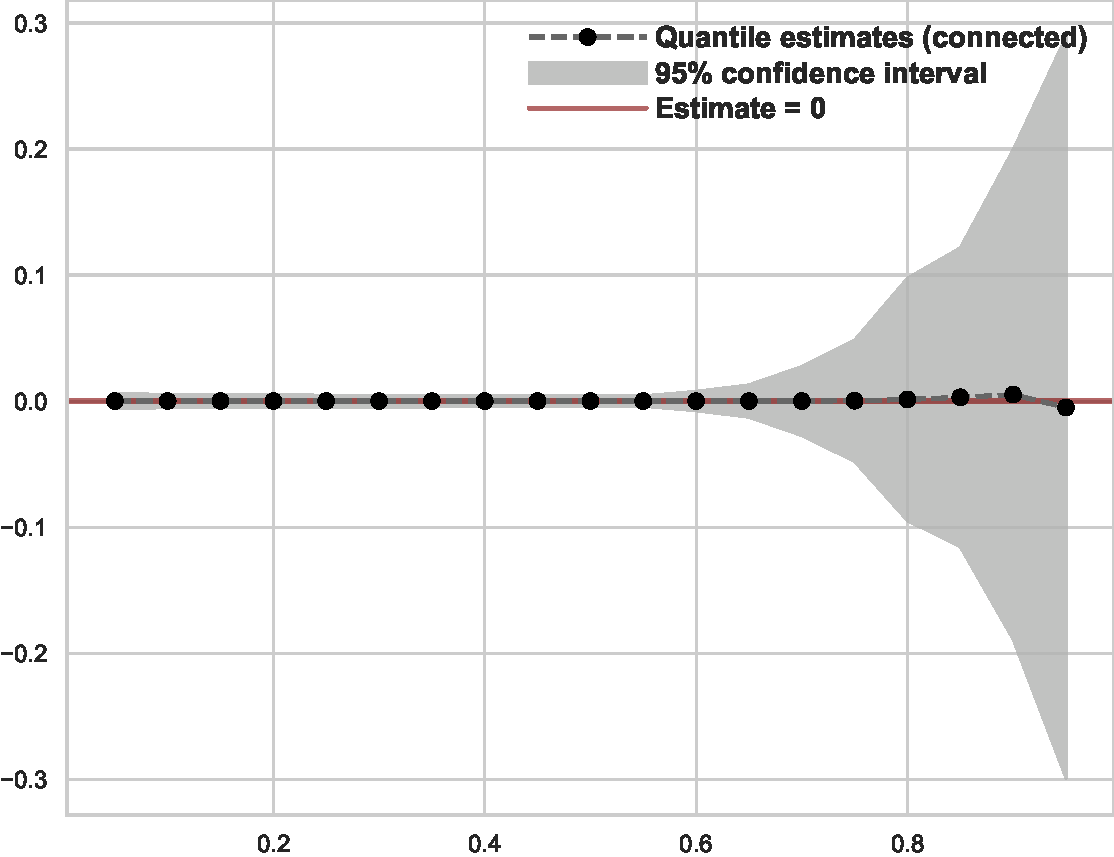
\includegraphics[width=.55\linewidth]{../figs/quantile_reg_covariates_duration_adult.pdf}
	\caption*{\footnotesize \emph{Notes:} 
		Dependent variable is the number of hours panelists in our sample spent on adult sites.
		Each point indicates the difference between Republicans and Democrats and corresponds to a quantile regression at the quantile indicated by the x-axis.
		Covariates included on the right-hand side are: gender (Female/Male), race (White/Black/Hispanic/Asian/Others), education level (no HS/HS graduate/some college/college graduate), age and its quadratic, and region (NE/MW/S/W).
		95\% confidence intervals constructed from robust standard errors.
		See \cref{fig:quantile_regression_duration} for the same plot without covariates.
	}
	\label{fig:quantile_regression_duration_covariates}
\end{figure}

%==============================================================================
% Fig of quantile regression estimates
% Time Spent on Adult Sites by Party (for individuals who consumed pornography)
%==============================================================================
\begin{figure}[ht]
	\centering
	\caption{Quantile Estimates--Hours Spent on Adult Sites by Party (for individuals who consumed pornography)}
	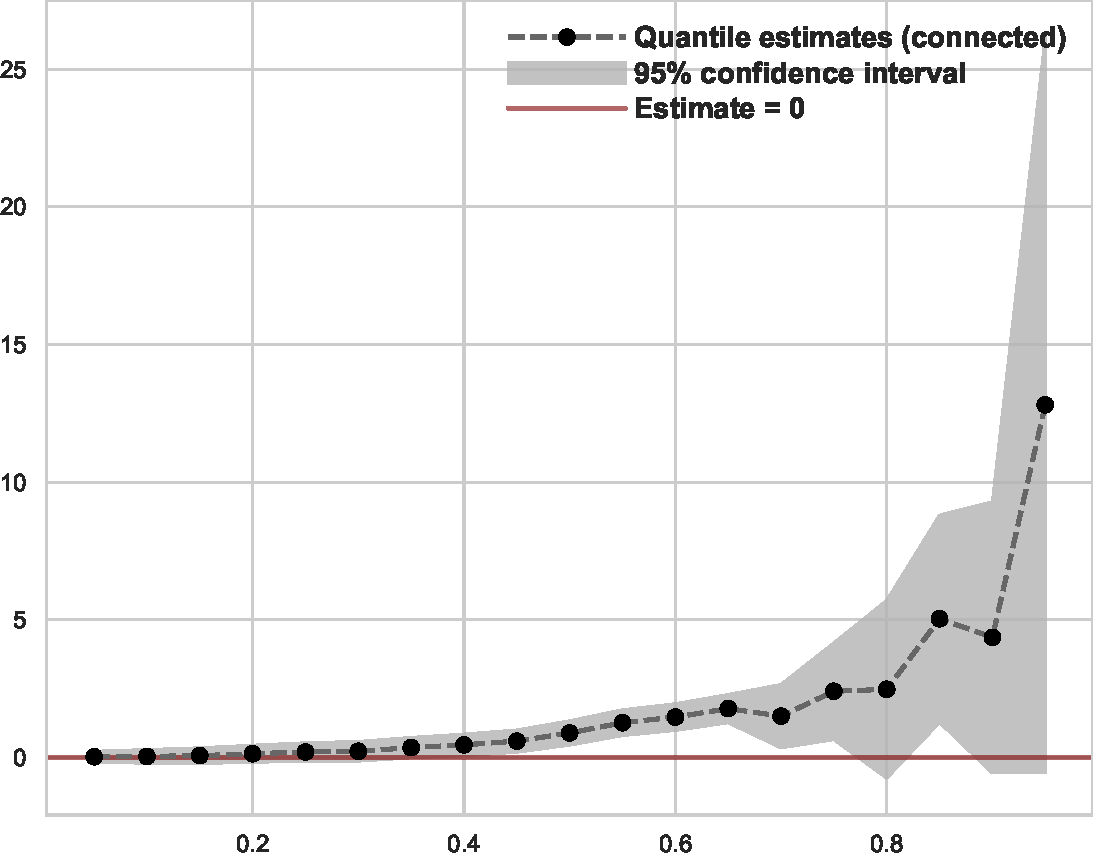
\includegraphics[width=.55\linewidth]{../figs/quantile_reg_nonzero_duration_adult.pdf}
	\caption*{\footnotesize \emph{Notes:} 
		Dependent variable is the number of hours panelists in our sample spent on adult sites.
		Each point indicates the difference between Republicans and Democrats and corresponds to a quantile regression at the quantile indicated by the x-axis.
		Only includes panelists who consumed pornography in the sample period.
		95\% confidence intervals constructed from robust standard errors.
		See \cref{fig:quantile_regression_duration} for the same plot for the full sample.
	}
	\label{fig:quantile_regression_duration_nonzeroes}
\end{figure}

%==============================================================================
% Fig of quantile regression estimates
% Time Spent on Adult Sites by Party (for individuals who consumed pornography and with covariates)
%==============================================================================
\begin{figure}[ht]
	\centering
	\caption{Quantile Estimates--Hours Spent on Adult Sites by Party (for individuals who consumed pornography and with covariates)}
	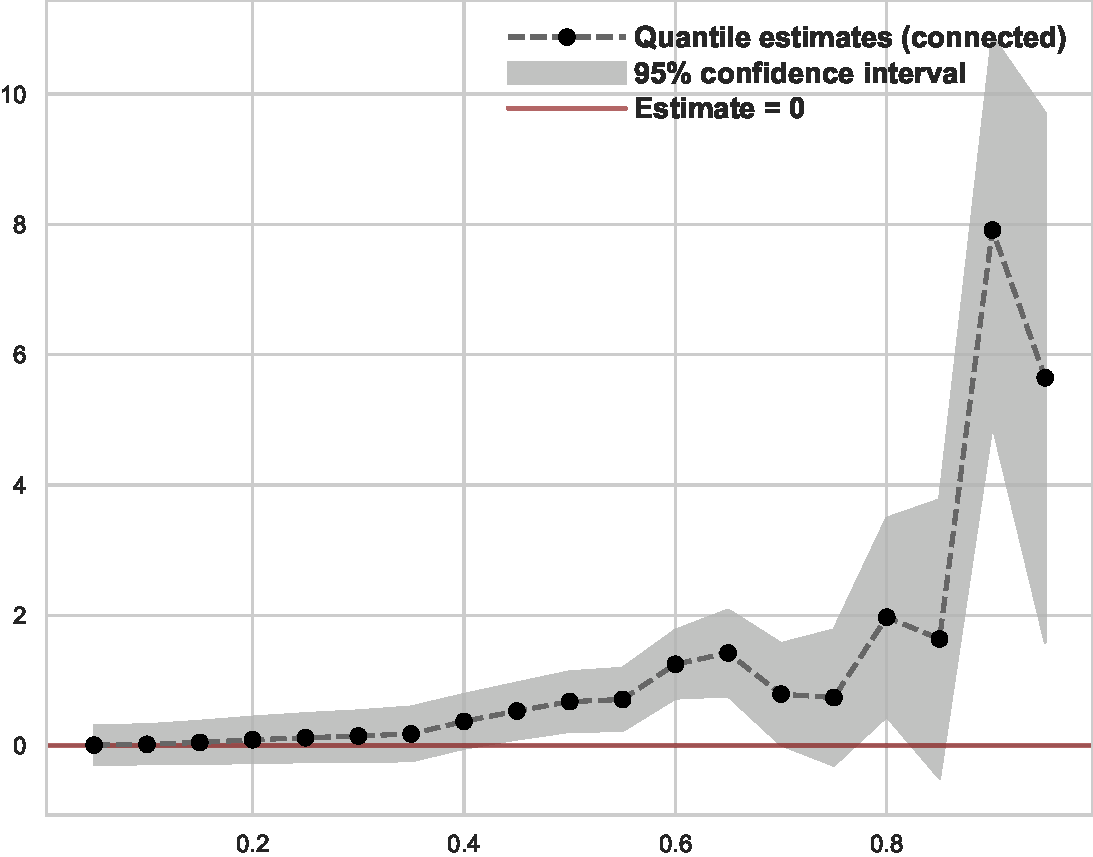
\includegraphics[width=.55\linewidth]{../figs/quantile_reg_nonzero_covariates_duration_adult.pdf}
	\caption*{\footnotesize \emph{Notes:} 
		Dependent variable is the number of hours panelists in our sample spent on adult sites.
		Each point indicates the difference between Republicans and Democrats and corresponds to a quantile regression at the quantile indicated by the x-axis.
		Only includes panelists who consumed pornography in the sample period.
		Covariates included on the right-hand side are: gender (Female/Male), race (White/Black/Hispanic/Asian/Others), education level (no HS/HS graduate/some college/college graduate), age and its quadratic, and region (NE/MW/S/W).
		95\% confidence intervals constructed from robust standard errors.
		See \cref{fig:quantile_regression_duration_covariates} for the same plot for the full sample.
	}
	\label{fig:quantile_regression_duration_nonzeroes_covariates}
\end{figure}






%================================================================
% Fig of quantile regression estimates
% Percentage Time Spent on Adult Sites by Party (with covariates) 
%================================================================
\begin{figure}[ht]
	\centering
	\caption{Quantile Estimates--Percentage of Time Spent on Adult Sites by Party (with covariates)}
	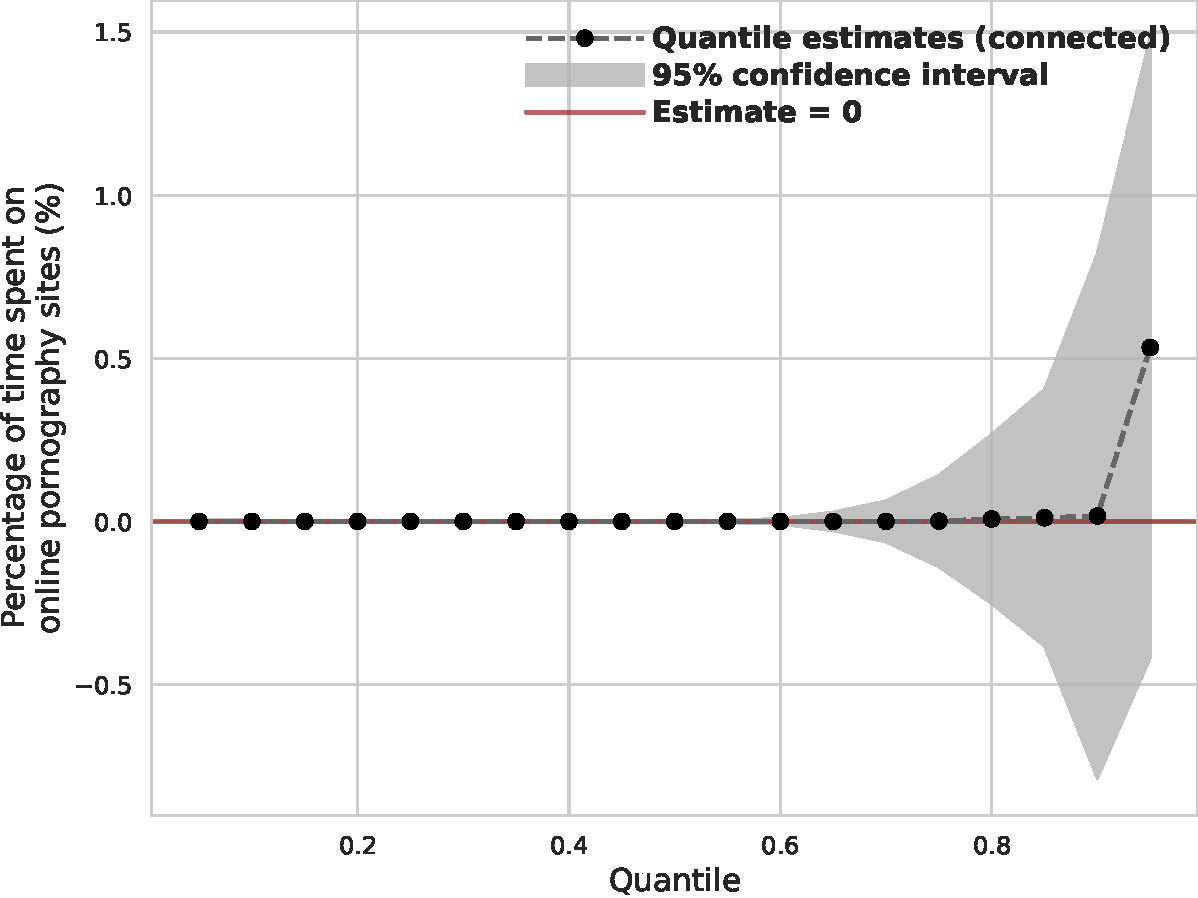
\includegraphics[width=.55\linewidth]{../figs/quantile_reg_covariates_proportion_duration_adult.pdf}
	\caption*{\footnotesize \emph{Notes:} 
		Dependent variable is the percentage of time panelists in our sample spent on adult sites.
		Each point indicates the difference between Republicans and Democrats and corresponds to a quantile regression at the quantile indicated by the x-axis.
		Covariates included on the right-hand side are: gender (Female/Male), race (White/Black/Hispanic/Asian/Others), education level (no HS/HS graduate/some college/college graduate), age and its quadratic, and region (NE/MW/S/W).
		95\% confidence intervals constructed from robust standard errors.
		See \cref{fig:quantile_regression_prop_duration} for the same plot without covariates.
	}
	\label{fig:quantile_regression_prop_duration_covariates}
\end{figure}

%==============================================================================
% Fig of quantile regression estimates
% Percentage Time Spent on Adult Sites by Party (for individuals who consumed pornography)
%==============================================================================
\begin{figure}[ht]
	\centering
	\caption{Quantile Estimates--Percentage of Time Spent on Adult Sites by Party (for individuals who consumed pornography)}
	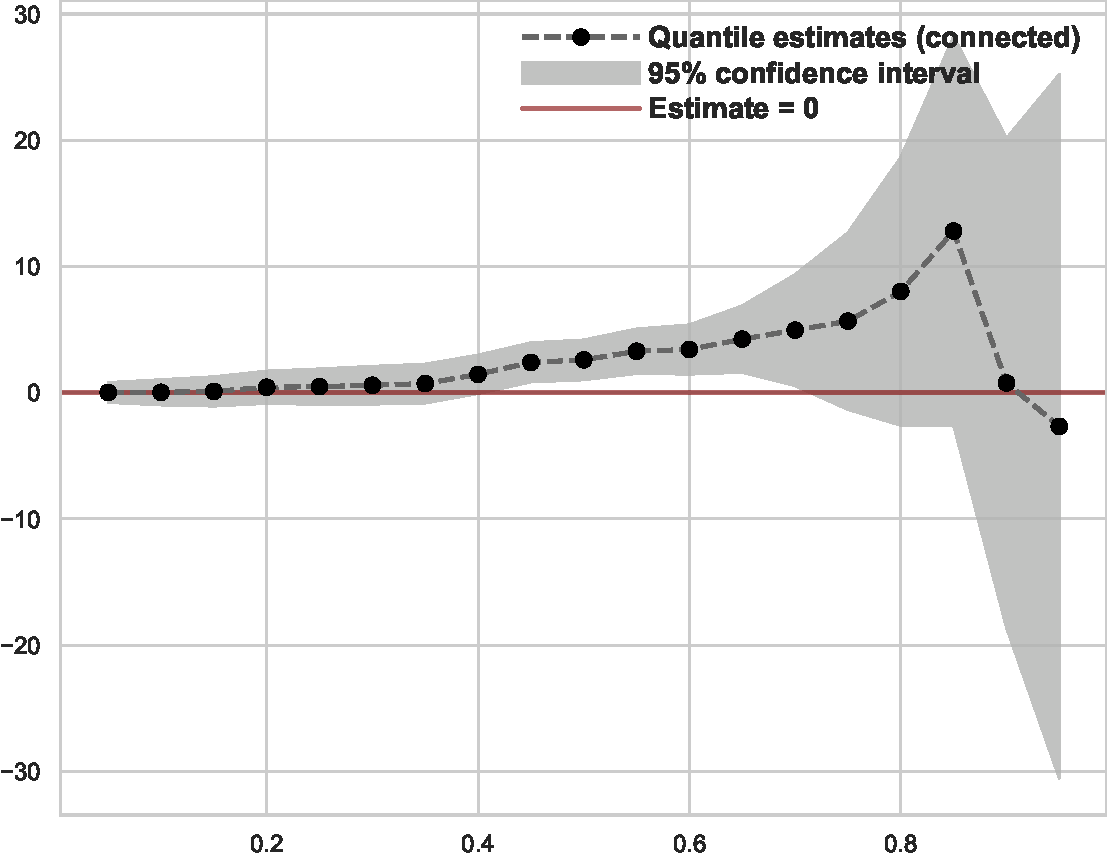
\includegraphics[width=.55\linewidth]{../figs/quantile_reg_nonzero_proportion_duration_adult.pdf}
	\caption*{\footnotesize \emph{Notes:} 
		Dependent variable is the percentage of time panelists in our sample spent on adult sites.
		Each point indicates the difference between Republicans and Democrats and corresponds to a quantile regression at the quantile indicated by the x-axis.
		Only includes panelists who consumed pornography in the sample period.
		95\% confidence intervals constructed from robust standard errors.
		See \cref{fig:quantile_regression_prop_duration} for the same plot for the full sample.
	}
	\label{fig:quantile_regression_prop_duration_nonzeroes}
\end{figure}

%==============================================================================
% Fig of quantile regression estimates
% Time Spent on Adult Sites by Party (for individuals who consumed pornography and with covariates)
%==============================================================================
\begin{figure}[ht]
	\centering
	\caption{Quantile Estimates--Percentage of Time Spent on Adult Sites by Party (for individuals who consumed pornography and with covariates)}
	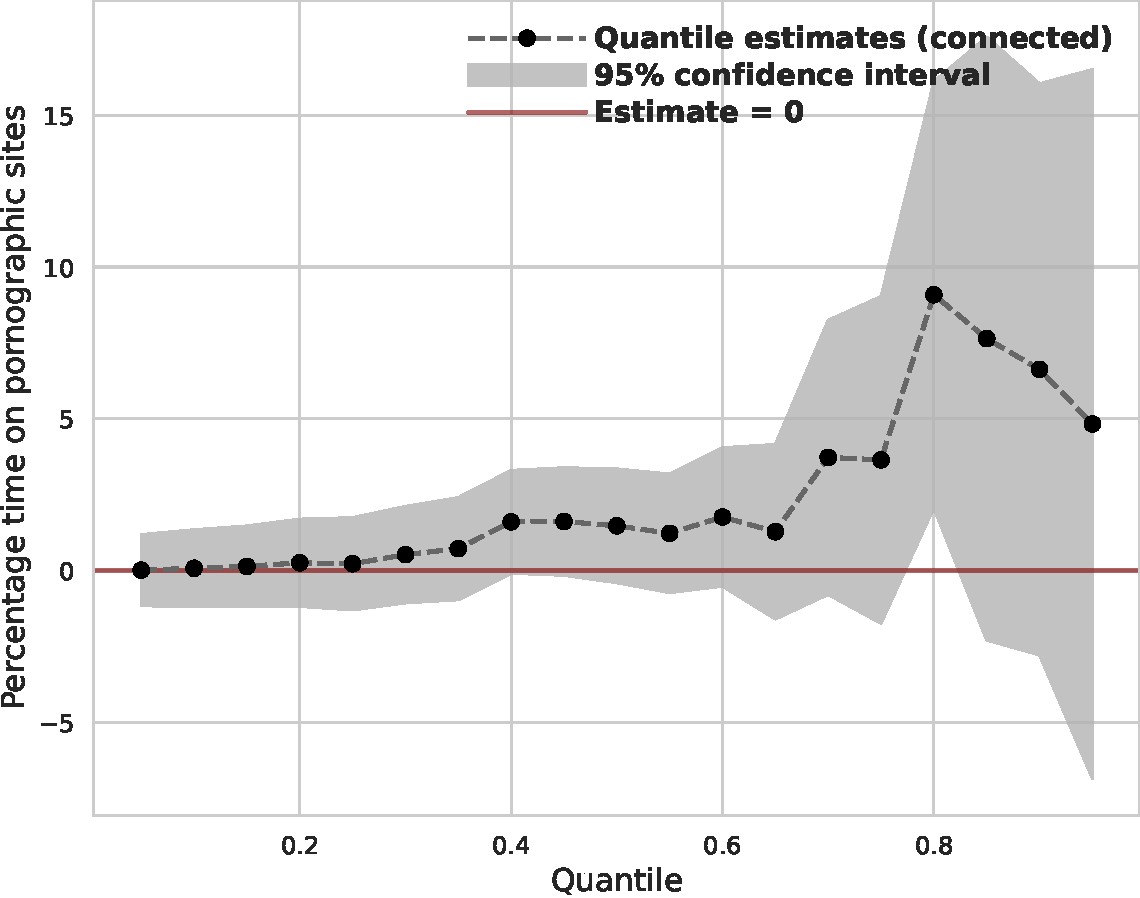
\includegraphics[width=.55\linewidth]{../figs/quantile_reg_nonzero_covariates_proportion_duration_adult.pdf}
	\caption*{\footnotesize \emph{Notes:} 
		Dependent variable is the percentage of time panelists in our sample spent on adult sites.
		Each point indicates the difference between Republicans and Democrats and corresponds to a quantile regression at the quantile indicated by the x-axis.
		Only includes panelists who consumed pornography in the sample period.
		Covariates included on the right-hand side are: gender (Female/Male), race (White/Black/Hispanic/Asian/Others), education level (no HS/HS graduate/some college/college graduate), age and its quadratic, and region (NE/MW/S/W).
		95\% confidence intervals constructed from robust standard errors.
		See \cref{fig:quantile_regression_prop_duration_covariates} for the same plot for the full sample.
	}
	\label{fig:quantile_regression_prop_duration_nonzeroes_covariates}
\end{figure}
\FloatBarrier

%===============================================================================
%===============================================================================
% Analogous results for visits to adult sites
%===============================================================================
%===============================================================================
\section{Analyses of Visits}
%=================================================
% Figure for Distribution of visits to adult sites
%=================================================
\begin{figure}[ht]
	\centering
	\caption{Distribution of Traffic to Pornography Online}
	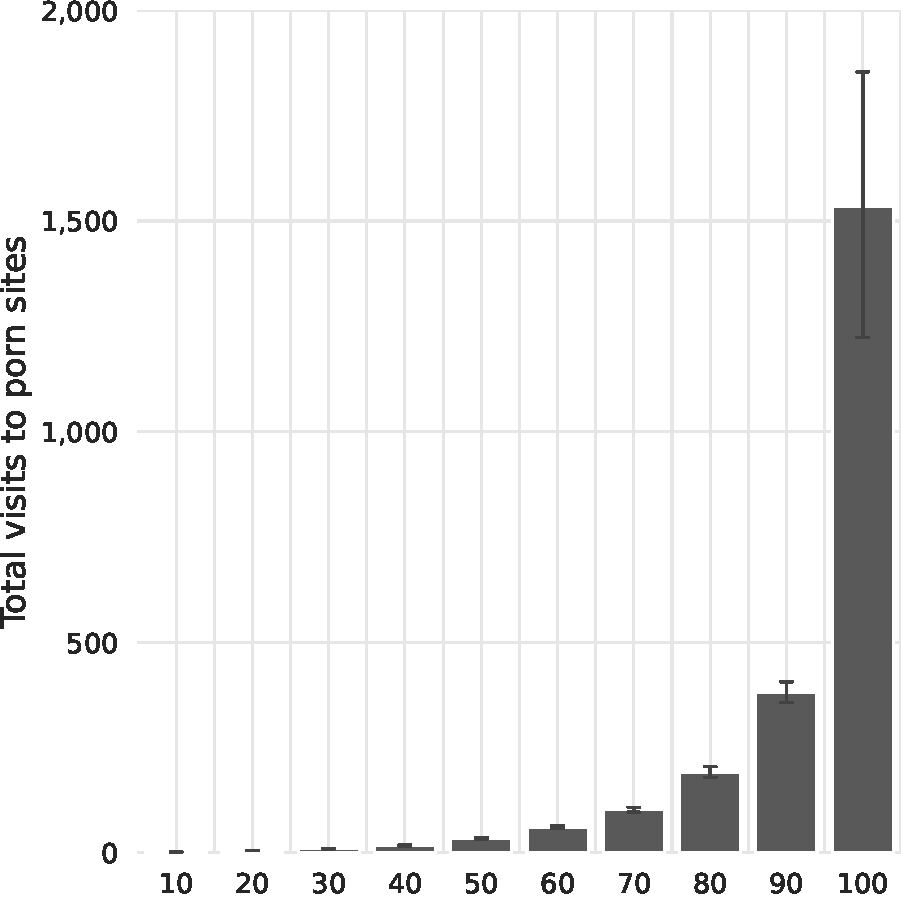
\includegraphics[width=.5\linewidth]{../figs/distribution_visits_to_adultsites.pdf}
	\caption*{\footnotesize \emph{Notes:} 
		Figure shows the number of visits to adult sites by individuals who consumed pornography in the sample period.
		Individuals are split into deciles with each bin containing approximately the same number of individuals.
		Height of bars indicate mean of each bin.
		Capped vertical bars are 95\% confidence intervals.
		See \cref{tab:distribution_visits} for the more tabulated values.
	}
	\label{fig:distribution_visits}
\end{figure}




%===============================================================
% Figure for Distribution of proportion of visits to adult sites
%===============================================================
\begin{figure}
	\centering
	\caption{Percentage of Traffic to Pornography Online}
	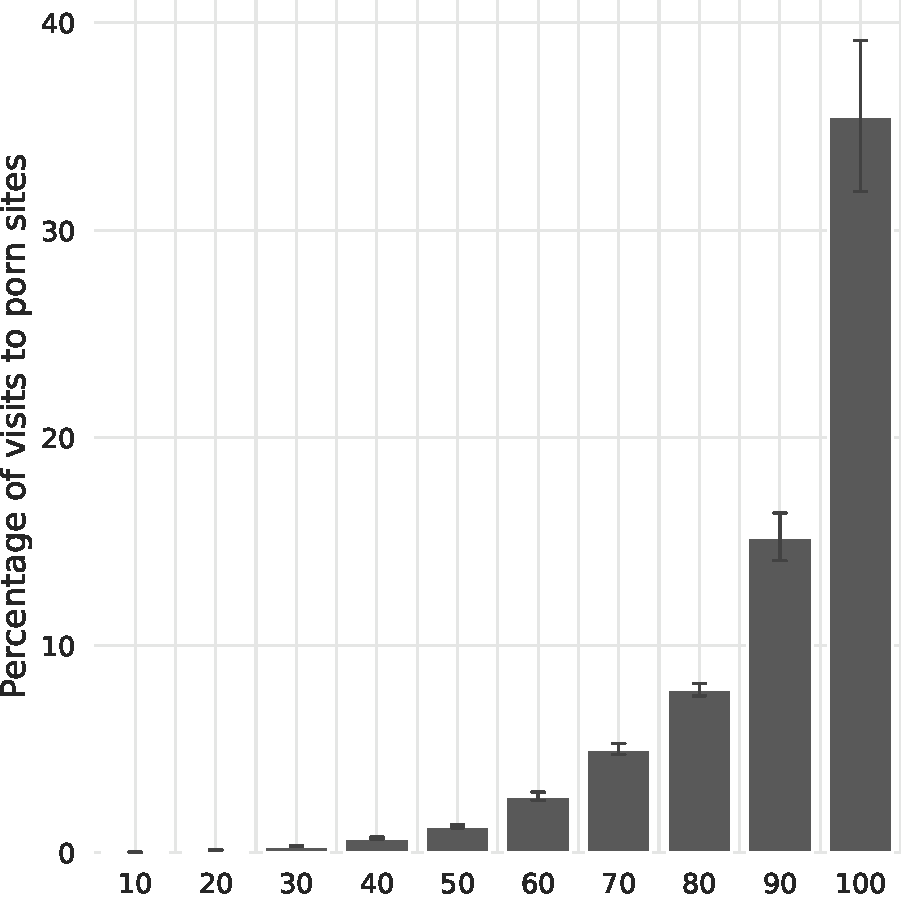
\includegraphics[width=.5\linewidth]{../figs/distribution_proportion_visits_to_adultsites.pdf}
	\caption*{\footnotesize \emph{Notes:} 
		Figure shows the proportion of visits to adult sites by individuals who consumed pornography in the sample period.
		Individuals are split into deciles with each bin containing approximately the same number of individuals.
		Height of bars indicate mean of each bin.
		Capped vertical bars are 95\% confidence intervals.
		See \cref{tab:distribution_prop_visits} for the more tabulated values.
	}
	\label{fig:distribution_prop_visits}
\end{figure}



%==========================================
% Splits by party for visits to adult sites
%==========================================
\begin{figure}
	\centering
	\caption{Distribution of Traffic to Pornography Online by Party}
	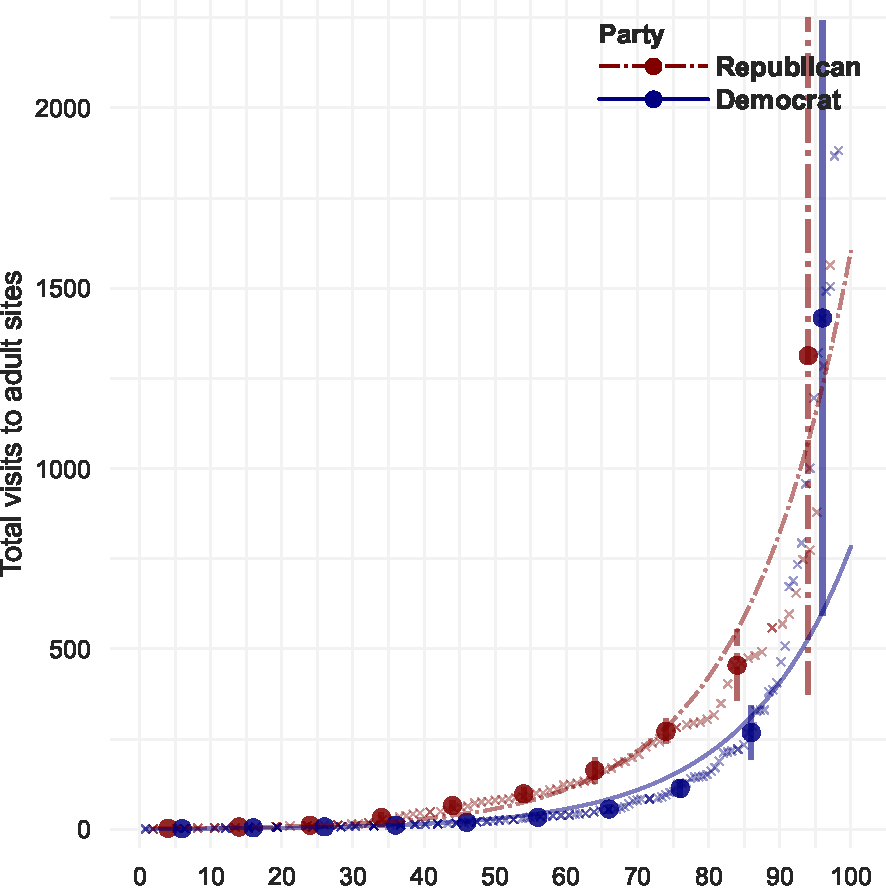
\includegraphics[width=.55\linewidth]{../figs/distribution_visits_to_adultsites_by_party.pdf}
	\caption*{\footnotesize \emph{Notes:} 
		Figure shows splits by party and by percentiles for visits to adult sites for panelists in the sample who consumed pornography in the sample period.
		Round markers and the corresponding vertical lines indicate the mean and 95\% confidence intervals for each bin.
		The \emph{x} symbols indicate actual panelists based on their percentiles.
		See \cref{tab:distribution_visits_party} for the more tabulated values.
	}
	\label{fig:distribution_visits_party}
\end{figure}




%========================================================
% Splits by party for proportion of visits to adult sites
%========================================================
\begin{figure}
	\centering
	\caption{Percentage of Traffic to Pornographic Sites by Party}
	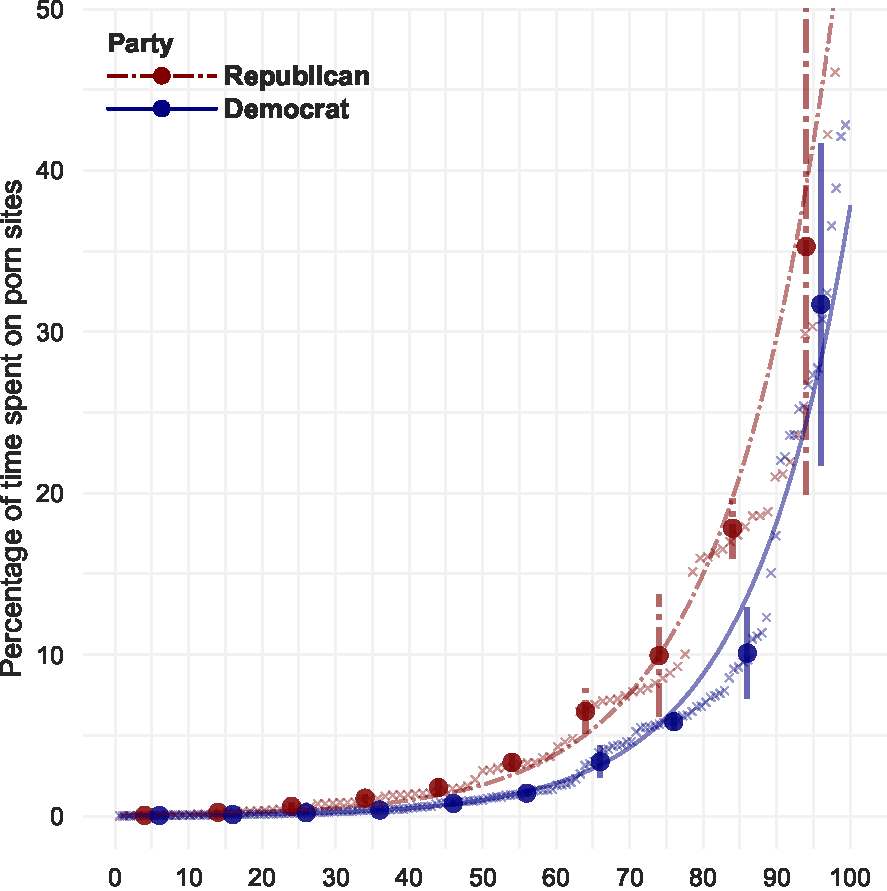
\includegraphics[width=.55\linewidth]{../figs/distribution_proportion_visits_to_adultsites_by_party.pdf}
	\caption*{\footnotesize \emph{Notes:} 
		Figure shows splits by party and by percentiles for visits to adult sites for panelists in the sample who consumed pornography in the sample period.
		Round markers and the corresponding vertical lines indicate the mean and 95\% confidence intervals for each bin.
		The \emph{x} symbols indicate actual panelists based on their percentiles.
		See \cref{tab:distribution_prop_visits_party} for the more tabulated values.
	}
	\label{fig:distribution_prop_visits_party}
\end{figure}



%===============================================
% Tabulated percentiles of visits to adult sites
%===============================================
\begin{table} \centering \small \setlength\tabcolsep{10 pt}
	\caption{Distribution of Traffic to Pornography Online}
	\label{tab:distribution_visits}
	\begin{adjustbox}{max width=\textwidth}
		\begin{tabular}{cr}
			\toprule
			\multicolumn{1}{c}{\textbf{Percentile}}&\multicolumn{1}{c}{\textbf{Hours}}\\
			\midrule
			0.00 &    1 \\
0.10 &    4 \\
0.20 &    7 \\
0.30 &   12 \\
0.40 &   25 \\
0.50 &   46 \\
0.60 &   77 \\
0.70 &  134 \\
0.80 &  262 \\
0.90 &  524 \\
0.95 & 1158 \\
0.96 & 1459 \\
0.97 & 1841 \\
0.98 & 2315 \\
0.99 & 2830 \\
1.00 & 4264 \\
			\bottomrule
		\end{tabular}
	\end{adjustbox}
	\caption*{\footnotesize \emph{Notes:} 
		Table shows key percentiles (each of the ten deciles plus quantiles at the right tail) and their corresponding values for traffic to porn sites by individuals who consumed pornography in the sample period. 
		See \cref{fig:distribution_visits} for the plot.
	}
\end{table}


%=============================================================
% Tabulated percentiles of proportion of visits to adult sites
%=============================================================
\begin{table} \centering \small \setlength\tabcolsep{10 pt}
	\caption{Percentage of Traffic to Pornographic Sites}
	\label{tab:distribution_prop_visits}
	\begin{adjustbox}{max width=\textwidth}
		\begin{tabular}{cr}
			\toprule
			\multicolumn{1}{c}{\textbf{Percentile}}&\multicolumn{1}{c}{\textbf{Hours}}\\
			\midrule
			0.00 &  0.0 \\
0.10 &  0.1 \\
0.20 &  0.2 \\
0.30 &  0.5 \\
0.40 &  1.0 \\
0.50 &  1.6 \\
0.60 &  3.7 \\
0.70 &  6.3 \\
0.80 &  9.7 \\
0.90 & 22.0 \\
0.95 & 31.4 \\
			\bottomrule
		\end{tabular}
	\end{adjustbox}
	\caption*{\footnotesize \emph{Notes:} 
		Table shows key percentiles (each of the ten deciles plus quantiles at the right tail) and their corresponding values for traffic to porn sites by individuals who consumed pornography in the sample period. 
		See \cref{fig:distribution_prop_visits} for the plot.
	}
\end{table}


%======================================================================
% Tabulated splits by party and by percentiles for visits to adultsites
%======================================================================
\begin{table} \centering \small \setlength\tabcolsep{10 pt}
	\caption{Distribution of Traffic to Pornography Online by Party}
	\label{tab:distribution_visits_party}
	\begin{adjustbox}{max width=\textwidth}
		\begin{tabular}{crr}
			\toprule
			\multicolumn{1}{l}{\textbf{Percentile}}&\multicolumn{1}{c}{\textbf{Republicans}}&\multicolumn{1}{r}{\textbf{Democrats}}\\
			\midrule
			0.00 &     1 &     1 \\
0.10 &     4 &     2 \\
0.20 &     9 &     5 \\
0.30 &    15 &     9 \\
0.40 &    48 &    14 \\
0.50 &    82 &    25 \\
0.60 &   125 &    39 \\
0.70 &   210 &    82 \\
0.80 &   310 &   157 \\
0.90 &   566 &   452 \\
0.95 &   863 & 1,246 \\
0.96 & 1,235 & 1,425 \\
0.97 & 1,539 & 1,503 \\
0.98 & 2,348 & 1,875 \\
0.99 & 2,414 & 2,465 \\
1.00 & 2,560 & 3,980 \\
			\bottomrule
		\end{tabular}
	\end{adjustbox}
	\caption*{\footnotesize \emph{Notes:} 
		Table shows splits by party and by key percentiles (each of the ten deciles plus quantiles at the right tail) for traffic to porn sites by individuals who consumed pornography in the sample period. See \cref{fig:distribution_visits_party} for the plot.
	}
\end{table}


%===============================================================================
% Tabulated splits by party and by percentiles for proportion of time spent on adultsites
%===============================================================================
\begin{table} \centering \small \setlength\tabcolsep{10 pt}
	\caption{Percentage of Traffic to Pornographic Sites by Party}
	\label{tab:distribution_prop_visits_party}
	\begin{adjustbox}{max width=\textwidth}
		\begin{tabular}{@{\hspace{0\tabcolsep}}ccc@{\hspace{0\tabcolsep}}}
			\toprule
			\multicolumn{1}{l}{\textbf{Percentile}}&\multicolumn{1}{c}{\textbf{Republicans}}&\multicolumn{1}{r}{\textbf{Democrats}}\\
			\midrule
			0.00 &  0.0 &  0.0 \\
0.10 &  0.1 &  0.1 \\
0.20 &  0.4 &  0.1 \\
0.30 &  0.8 &  0.3 \\
0.40 &  1.4 &  0.5 \\
0.50 &  2.8 &  1.0 \\
0.60 &  4.3 &  1.9 \\
0.70 &  7.7 &  4.6 \\
0.80 & 16.0 &  7.0 \\
0.90 & 21.1 & 18.8 \\
0.95 & 30.5 & 27.4 
% 0.96 & 32.7 & 29.9 \\
% 0.97 & 42.6 & 33.6 \\
% 0.98 & 46.5 & 38.6 \\
% 0.99 & 52.8 & 42.4 \\
% 1.00 & 53.5 & 59.9 \\
			\bottomrule
		\end{tabular}
	\end{adjustbox}
	\caption*{\footnotesize \emph{Notes:} 
		Table shows splits by party and by key percentiles (each of the ten deciles plus quantiles at the right tail) for traffic to porn sites by individuals who consumed pornography in the sample period. See \cref{fig:distribution_prop_visits_party} for the plot.
	}
\end{table}


%=======================
% Quantile regressions
% Traffic to adult sites
%=======================
\begin{figure}
	\centering
	\caption{Quantile Estimates--Traffic to Adult Sites by Party}
	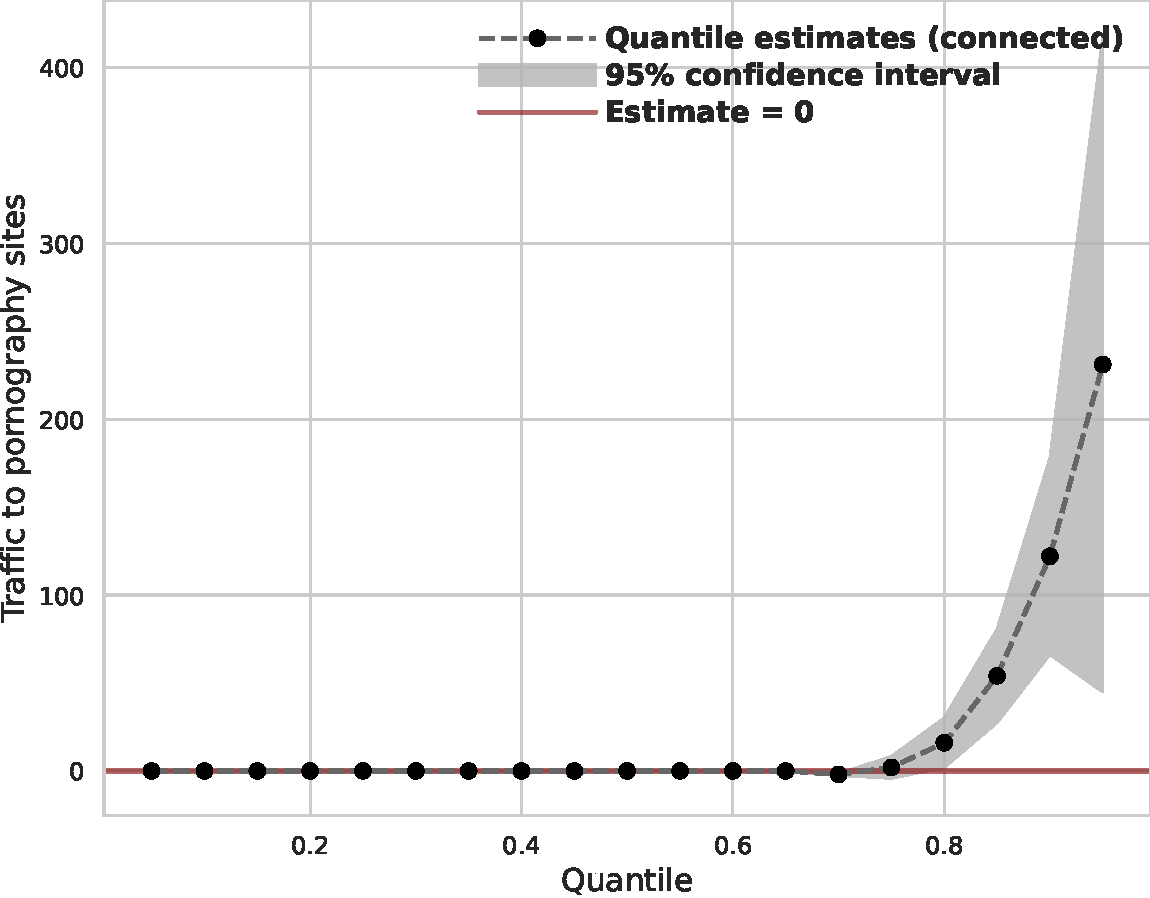
\includegraphics[width=.6\linewidth]{../figs/quantile_reg_visits_adult.pdf}
	\caption*{\footnotesize \emph{Notes:} 
		Dependent variable is the number of visits to porn sites by panelists in our sample.
		Each point indicates the difference between Republicans and Democrats and corresponds to a quantile regression at the quantile indicated by the x-axis.
		95\% confidence intervals constructed from robust standard errors.
		See \cref{fig:quantile_regression_visits_covariates} for the same plot controlling for individual characteristics.
	}
	\label{fig:quantile_regression_visits}
\end{figure}

%=====================================
% Quantile regressions
% Proportion of traffic to adult sites
%=====================================
\begin{figure}
	\centering
	\caption{Quantile Estimates--Percentage of Traffic to Adult Sites by Party}
	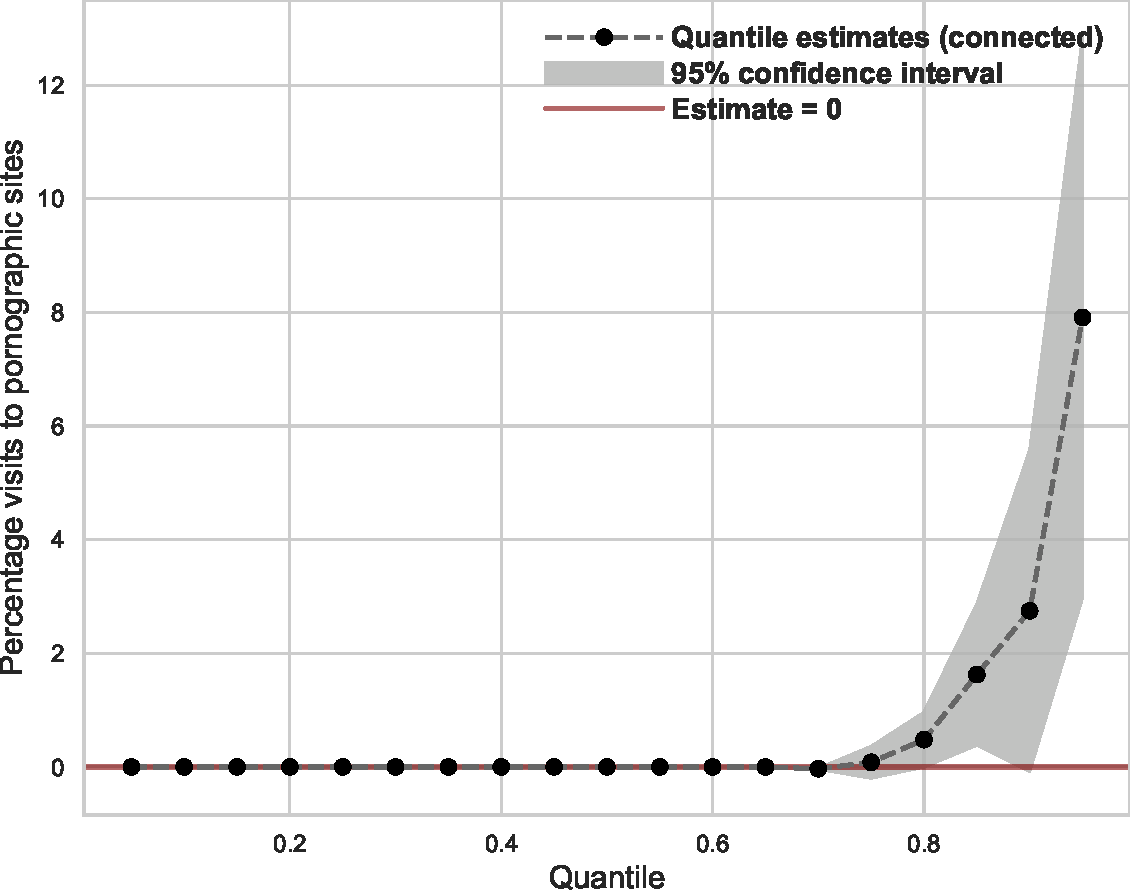
\includegraphics[width=.6\linewidth]{../figs/quantile_reg_proportion_visits_adult.pdf}
	\caption*{\footnotesize \emph{Notes:} 
		Dependent variable is the percentage of traffic to porn sites by panelists in our sample.
		Each point indicates the difference between Republicans and Democrats and corresponds to a quantile regression at the quantile indicated by the x-axis.
		95\% confidence intervals constructed from robust standard errors.
		See \cref{fig:quantile_regression_prop_visits_covariates} for the same plot controlling for individual characteristics.
	}
	\label{fig:quantile_regression_prop_visits}
\end{figure}


%==================================================
% Fig of quantile regression estimates
% Traffic to Adult Sites by Party (with covariates) 
%==================================================
\begin{figure}
	\centering
	\caption{Quantile Estimates--Traffic to Porn Sites by Party (with covariates)}
	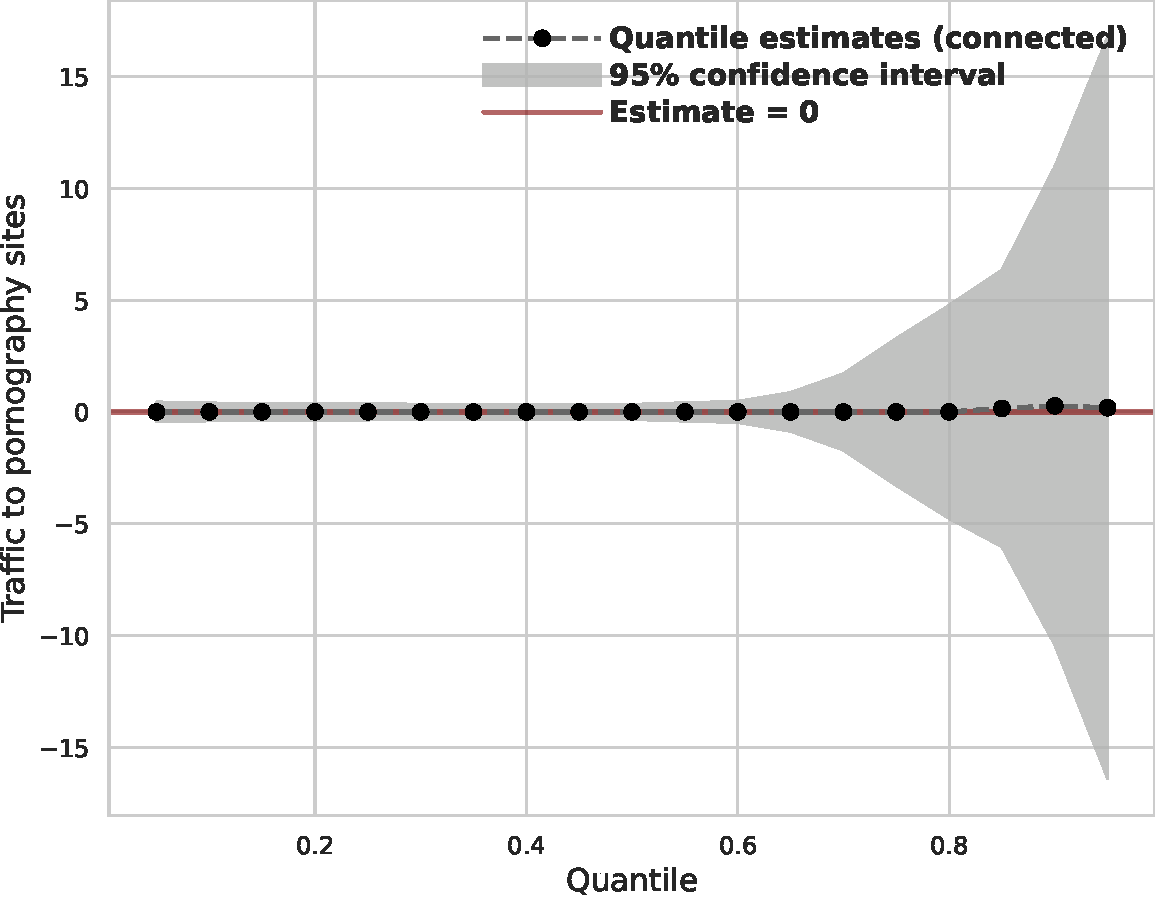
\includegraphics[width=.55\linewidth]{../figs/quantile_reg_covariates_visits_adult.pdf}
	\caption*{\footnotesize \emph{Notes:} 
		Dependent variable is the number of visits to porn sites by panelists in our sample.
		Each point indicates the difference between Republicans and Democrats and corresponds to a quantile regression at the quantile indicated by the x-axis.
		Covariates included on the right-hand side are: gender (Female/Male), race (White/Black/Hispanic/Asian/Others), education level (no HS/HS graduate/some college/college graduate), age and its quadratic, and region (NE/MW/S/W).
		95\% confidence intervals constructed from robust standard errors.
		See \cref{fig:quantile_regression_visits} for the same plot without covariates.
	}
	\label{fig:quantile_regression_visits_covariates}
\end{figure}


%===========================================================================
% Fig of quantile regression estimates
% Traffic to Adult Sites by Party (for individuals who consumed pornography)
%===========================================================================
\begin{figure}
	\centering
	\caption{Quantile Estimates--Traffic to Porn Sites by Party (for individuals who consumed pornography)}
	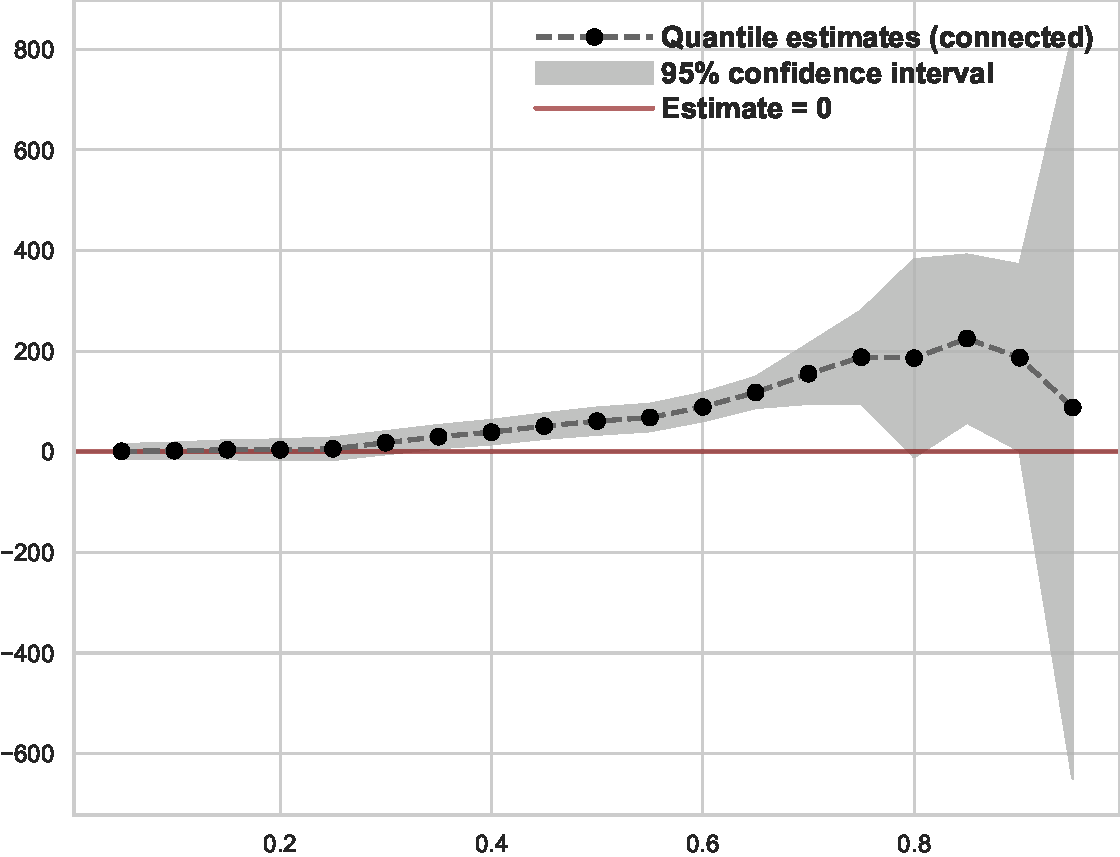
\includegraphics[width=.55\linewidth]{../figs/quantile_reg_nonzero_visits_adult.pdf}
	\caption*{\footnotesize \emph{Notes:} 
		Dependent variable is the number of visits to porn sites by panelists in our sample.
		Each point indicates the difference between Republicans and Democrats and corresponds to a quantile regression at the quantile indicated by the x-axis.
		Only includes panelists who consumed pornography in the sample period.
		95\% confidence intervals constructed from robust standard errors.
		See \cref{fig:quantile_regression_visits} for the same plot for the full sample.
	}
	\label{fig:quantile_regression_visits_nonzeroes}
\end{figure}


%==============================================================================
% Fig of quantile regression estimates
% Traffic to Adult Sites by Party (for individuals who consumed pornography and with covariates)
%==============================================================================
\begin{figure}
	\centering
	\caption{Quantile Estimates--Traffic to Porn Sites by Party (for individuals who consumed pornography and with covariates)}
	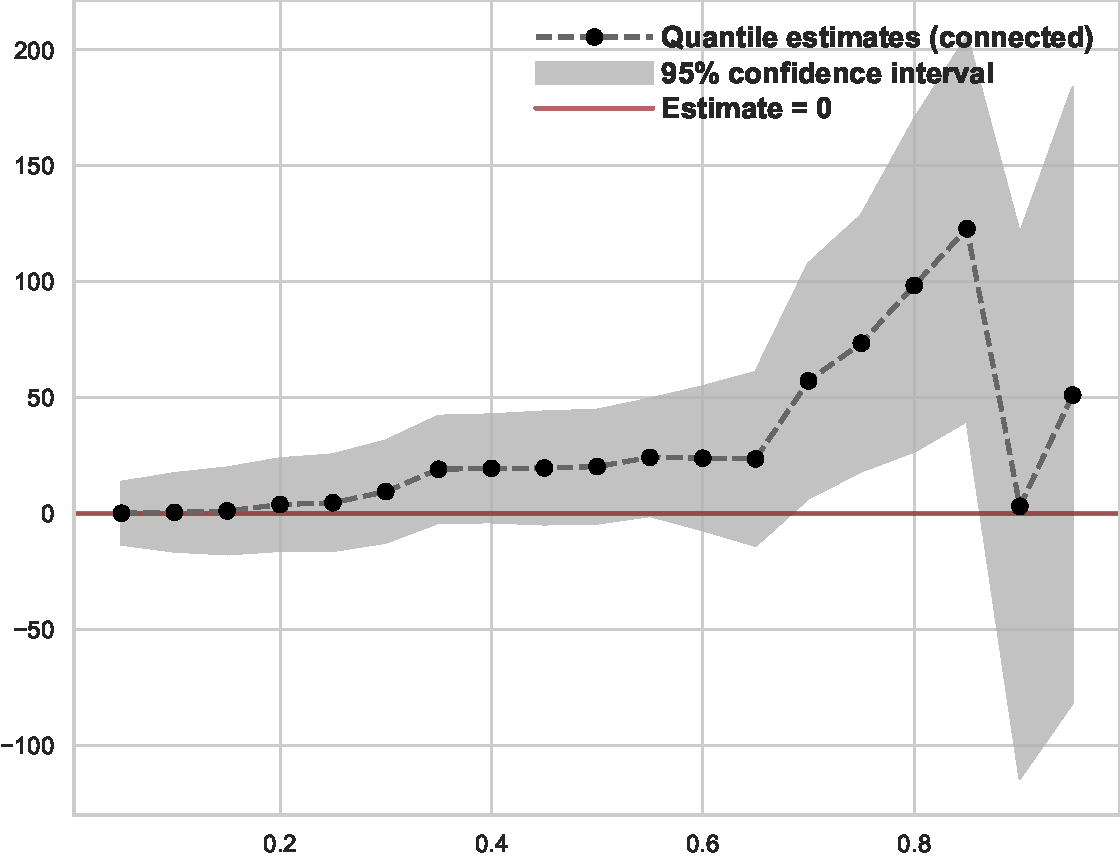
\includegraphics[width=.55\linewidth]{../figs/quantile_reg_nonzero_covariates_visits_adult.pdf}
	\caption*{\footnotesize \emph{Notes:} 
		Dependent variable is the number of visits to porn sites by panelists in our sample.
		Each point indicates the difference between Republicans and Democrats and corresponds to a quantile regression at the quantile indicated by the x-axis.
		Only includes panelists who consumed pornography in the sample period.
		Covariates included on the right-hand side are: gender (Female/Male), race (White/Black/Hispanic/Asian/Others), education level (no HS/HS graduate/some college/college graduate), age and its quadratic, and region (NE/MW/S/W).
		95\% confidence intervals constructed from robust standard errors.
		See \cref{fig:quantile_regression_visits_covariates} for the same plot for the full sample.
	}
	\label{fig:quantile_regression_visits_nonzeroes_covariates}
\end{figure}




%=============================================================
% Fig of quantile regression estimates
% Percentage Traffic to Adult Sites by Party (with covariates) 
%=============================================================
\begin{figure}
	\centering
	\caption{Quantile Estimates--Percentage of Traffic to Adult Sites by Party (with covariates)}
	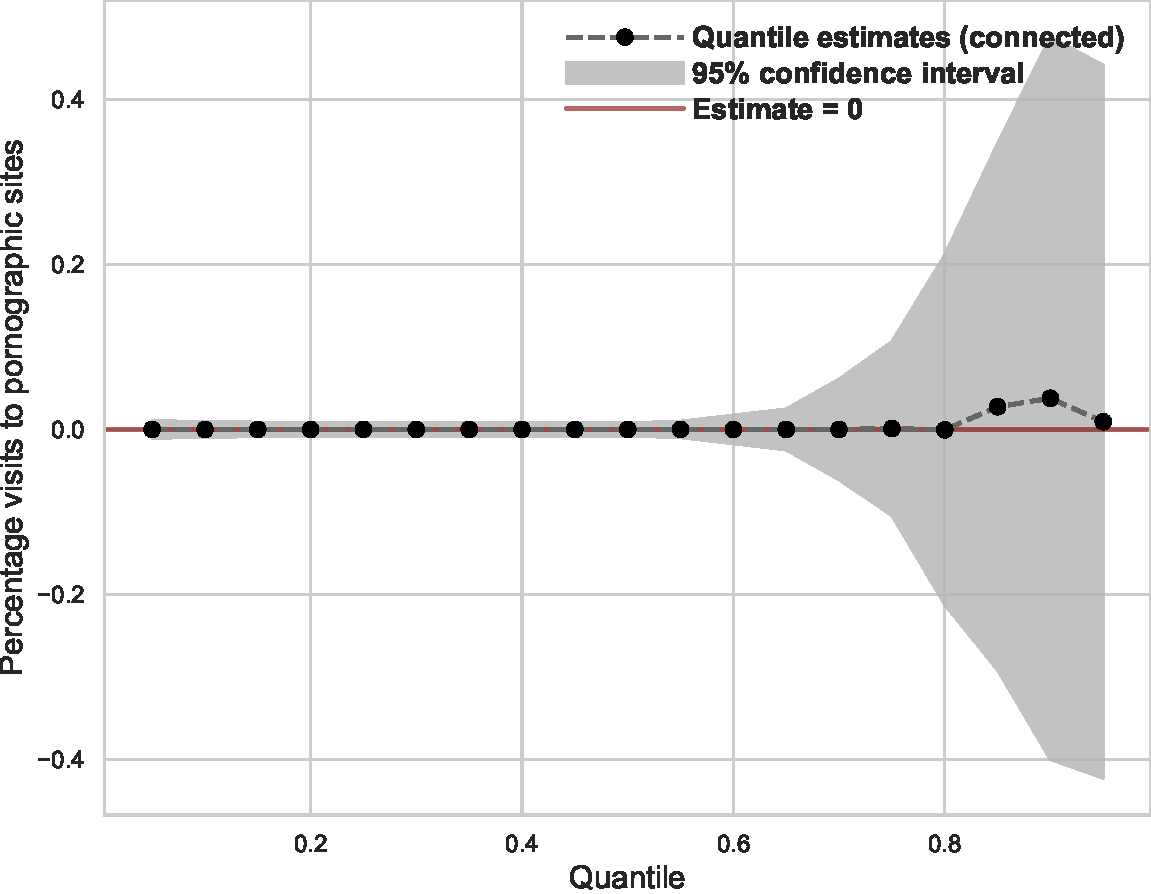
\includegraphics[width=.55\linewidth]{../figs/quantile_reg_covariates_proportion_visits_adult.pdf}
	\caption*{\footnotesize \emph{Notes:} 
		Dependent variable is the percentage of traffic to porn sites by panelists in our sample.
		Each point indicates the difference between Republicans and Democrats and corresponds to a quantile regression at the quantile indicated by the x-axis.
		Covariates included on the right-hand side are: gender (Female/Male), race (White/Black/Hispanic/Asian/Others), education level (no HS/HS graduate/some college/college graduate), age and its quadratic, and region (NE/MW/S/W).
		95\% confidence intervals constructed from robust standard errors.
		See \cref{fig:quantile_regression_prop_visits} for the same plot without covariates.
	}
	\label{fig:quantile_regression_prop_visits_covariates}
\end{figure}

%==============================================================================
% Fig of quantile regression estimates
% Percentage Traffic to Adult Sites by Party (for individuals who consumed pornography)
%==============================================================================
\begin{figure}
	\centering
	\caption{Quantile Estimates--Percentage of Traffic to Adult Sites by Party (for individuals who consumed pornography)}
	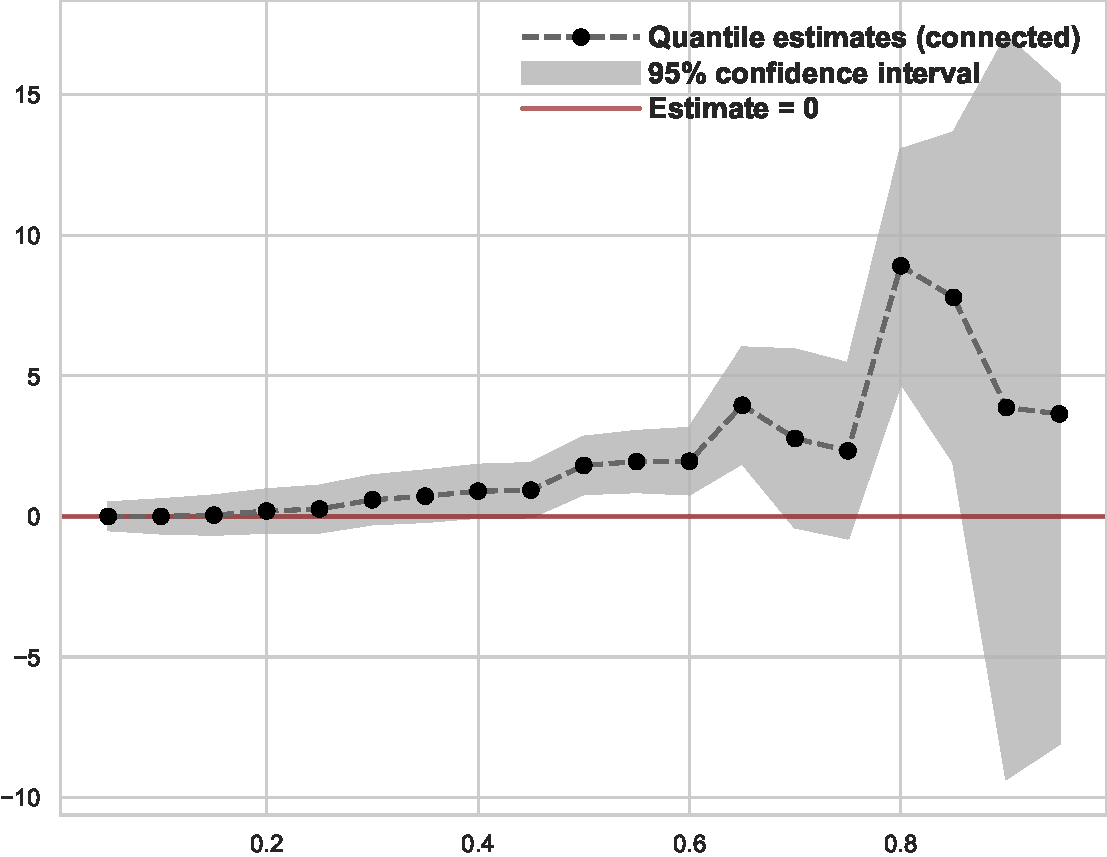
\includegraphics[width=.55\linewidth]{../figs/quantile_reg_nonzero_proportion_visits_adult.pdf}
	\caption*{\footnotesize \emph{Notes:} 
		Dependent variable is the percentage of traffic to porn sites by panelists in our sample.
		Each point indicates the difference between Republicans and Democrats and corresponds to a quantile regression at the quantile indicated by the x-axis.
		Only includes panelists who consumed pornography in the sample period.
		95\% confidence intervals constructed from robust standard errors.
		See \cref{fig:quantile_regression_prop_visits} for the same plot for the full sample.
	}
	\label{fig:quantile_regression_prop_visits_nonzeroes}
\end{figure}

%==============================================================================
% Fig of quantile regression estimates
% Percentage Traffic to Adult Sites by Party (for individuals who consumed pornography and with covariates)
%==============================================================================
\begin{figure}
	\centering
	\caption{Quantile Estimates--Percentage of Traffic to Adult Sites by Party (for individuals who consumed pornography and with covariates)}
	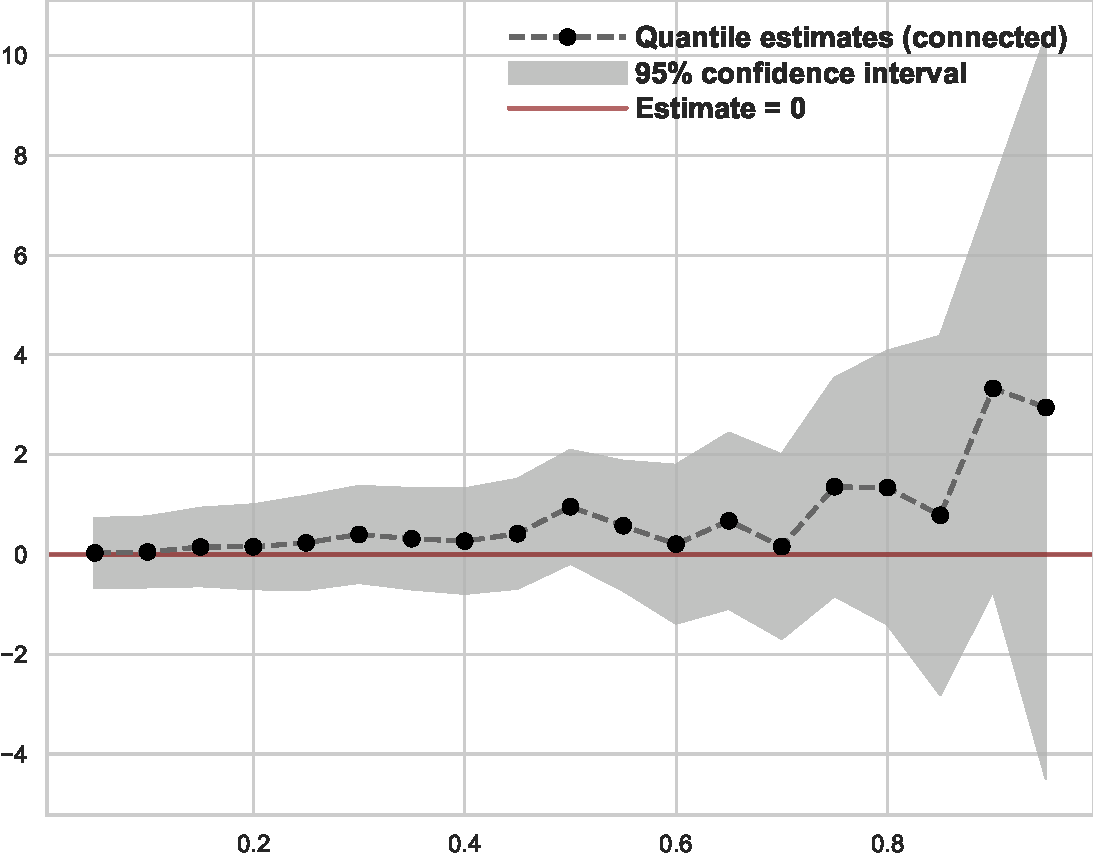
\includegraphics[width=.55\linewidth]{../figs/quantile_reg_nonzero_covariates_proportion_visits_adult.pdf}
	\caption*{\footnotesize \emph{Notes:} 
		Dependent variable is the percentage of traffic to porn sites by panelists in our sample.
		Each point indicates the difference between Republicans and Democrats and corresponds to a quantile regression at the quantile indicated by the x-axis.
		Only includes panelists who consumed pornography in the sample period.
		Covariates included on the right-hand side are: gender (Female/Male), race (White/Black/Hispanic/Asian/Others), education level (no HS/HS graduate/some college/college graduate), age and its quadratic, and region (NE/MW/S/W).
		95\% confidence intervals constructed from robust standard errors.
		See \cref{fig:quantile_regression_prop_visits_covariates} for the same plot for the full sample.
	}
	\label{fig:quantile_regression_prop_visits_nonzeroes_covariates}
\end{figure}

\end{document}
